\FloatBarrier
\section{Appendix}
\label{sec:appendix}

\begin{figure}[t]
  \centering
  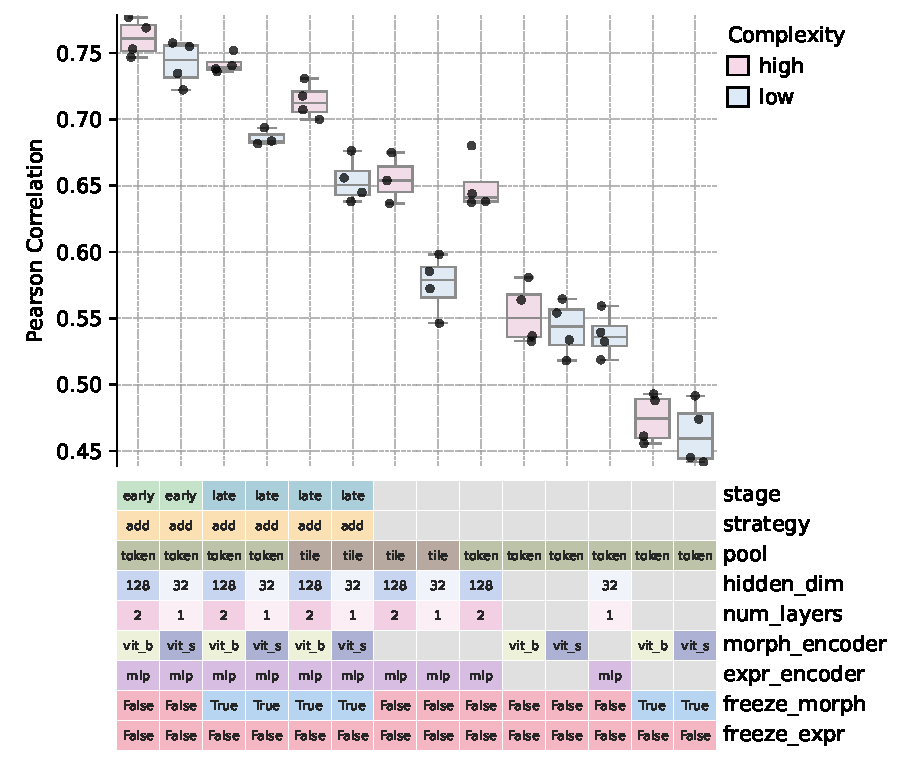
\includegraphics[width=0.75\textwidth]{figures/cell-pcc-low-high-boxplot-marsilea.pdf}
  \caption{\textbf{High- vs.\ low-capacity model comparison for cell type prediction.} Pearson correlation for low-capacity (ViT-S, single-layer MLP) and high-capacity (ViT-B, two-layer MLP) configurations across all fusion strategies. Increasing model capacity consistently benefits multimodal and expression-only models but provides no gain for morphology-only baselines.}
  \label{fig:p-fus:high-low-capacity}
\end{figure}

% $\downarrow$
% $\uparrow$
\begin{sidewaystable}
  \centering
  \scriptsize
\caption{Hyperparameter settings for all evaluated models on the gene prediction task. Entries marked with \{*\} indicate runs that did not converge.}
\label{tab:p-fus:gene-table}
\begin{tabular}{lllrlrllll}
\toprule
stage & strategy & morph\_encoder & freeze\_morph & expr\_encoder & freeze\_expr & pool & spearman $\uparrow$ & pearson $\uparrow$ & mse $\downarrow$\\
\midrule
early & add & vit\_small\_patch16\_224 & False & mlp & False & token & 0.811±0.017 & 0.820±0.013 & 0.705±0.030 \\
early & add & vit\_small\_patch16\_224 & True & mlp & False & token & 0.771±0.014 & 0.777±0.011 & 0.862±0.018 \\
early & concat & vit\_small\_patch16\_224 & False & mlp & False & token & 0.809±0.017 & 0.818±0.013 & 0.768±0.058 \\
late & add & conch & True & geneformer & True & tile & 0.727±0.017 & 0.747±0.012 & 0.979±0.014 \\
late & add & conch & True & mlp & False & tile & 0.752±0.012 & 0.763±0.008 & 0.942±0.028 \\
late & add & loki & True & geneformer & True & tile & 0.696±0.021 & 0.718±0.013 & 1.107±0.027 \\
late & add & loki & True & mlp & False & tile & 0.769±0.036 & 0.776±0.033 & 0.873±0.090 \\
late & add & phikon & True & geneformer & True & tile & 0.738±0.019 & 0.754±0.014 & 0.966±0.012 \\
late & add & phikon & True & mlp & False & tile & 0.787±0.013 & 0.796±0.011 & 0.799±0.011 \\
late & add & vit\_small\_patch16\_224 & False & geneformer & True & tile & 0.684±0.023 & 0.700±0.017 & 1.177±0.018 \\
late & add & vit\_small\_patch16\_224 & False & mlp & False & tile & 0.728±0.018 & 0.741±0.015 & 1.057±0.040 \\
late & add & vit\_small\_patch16\_224 & False & mlp & False & token & 0.773±0.016 & 0.778±0.014 & 0.887±0.029 \\
late & add & vit\_small\_patch16\_224 & True & geneformer & True & tile & 0.715±0.019 & 0.735±0.012 & 1.030±0.022 \\
late & add & vit\_small\_patch16\_224 & True & mlp & False & tile & 0.797±0.012 & 0.805±0.009 & 0.767±0.007 \\
late & add & vit\_small\_patch16\_224 & True & mlp & False & token & 0.813±0.010 & 0.819±0.007 & 0.706±0.008 \\
late & concat & conch & True & geneformer & True & tile & 0.738±0.018 & 0.756±0.013 & 0.950±0.011 \\
late & concat & conch & True & mlp & False & tile & 0.778±0.026 & 0.788±0.023 & 0.834±0.076 \\
late & concat & loki & True & geneformer & True & tile & 0.707±0.022 & 0.728±0.015 & 1.075±0.030 \\
late & concat & loki & True & mlp & False & tile & 0.781±0.020 & 0.788±0.018 & 0.825±0.034 \\
late & concat & phikon & True & geneformer & True & tile & 0.742±0.019 & 0.758±0.014 & 0.953±0.012 \\
late & concat & phikon & True & mlp & False & tile & 0.784±0.013 & 0.793±0.010 & 0.813±0.009 \\
late & concat & vit\_small\_patch16\_224 & False & geneformer & True & tile & 0.694±0.032 & 0.712±0.026 & 1.141±0.036 \\
late & concat & vit\_small\_patch16\_224 & False & mlp & False & tile & 0.740±0.019 & 0.752±0.016 & 1.011±0.031 \\
late & concat & vit\_small\_patch16\_224 & False & mlp & False & token & 0.786±0.016 & 0.791±0.013 & 0.829±0.021 \\
late & concat & vit\_small\_patch16\_224 & True & geneformer & True & tile & 0.722±0.018 & 0.742±0.012 & 1.007±0.019 \\
late & concat & vit\_small\_patch16\_224 & True & mlp & False & tile & 0.798±0.013 & 0.806±0.010 & 0.761±0.006 \\
late & concat & vit\_small\_patch16\_224 & True & mlp & False & token & 0.820±0.010 & 0.826±0.008 & 0.673±0.010 \\
- & - & conch & True & - & False & token & 0.626±0.017 & 0.631±0.018 & 1.359±0.026 \\
- & - & loki & True & - & False & token & 0.354±0.036 & 0.374±0.032 & 6.679±0.279 \\
- & - & phikon & True & - & False & token & 0.633±0.024 & 0.637±0.022 & 1.367±0.031 \\
- & - & vit\_small\_patch16\_224 & False & - & False & token & 0.648±0.028 & 0.654±0.026 & 1.332±0.037 \\
- & - & vit\_small\_patch16\_224 & True & - & False & token & 0.587±0.020 & 0.592±0.017 & 1.495±0.036 \\
- & - & - & False & geneformer & True & tile & 0.622±0.044 & 0.662±0.029 & 1.314±0.128 \\
- & - & - & False & mlp & False & token & 0.722±0.017 & 0.722±0.013 & 1.055±0.026 \\
\bottomrule
\end{tabular}
\end{sidewaystable}

% $\downarrow$
% $\uparrow$
\begin{sidewaystable}
  \centering
  \scriptsize
\caption{Hyperparameter settings for all evaluated models on the gene prediction task. Entries marked with \{*\} indicate runs that did not converge.}
\label{tab:p-fus:cell-table}

\begin{tabular}{lllrlrrlllll}
\toprule
stage & strategy & morph\_encoder & freeze\_morph & expr\_encoder & expr\_dim & freeze\_expr & pool & panel & spearman & pearson & mse \\
\midrule
early & add & vit\_small\_patch16\_224 & False & mlp & 32 & False & token & add & 0.606±0.021 & 0.688±0.020 & 0.424±0.028 \\
early & add & vit\_small\_patch16\_224 & True & mlp & 32 & False & token & add & 0.542±0.028 & 0.601±0.025 & 0.533±0.029 \\
late & add & vit\_small\_patch16\_224 & False & mlp & 32 & False & tile & add & 0.524±0.022 & 0.583±0.022 & 0.588±0.046 \\
late & add & vit\_small\_patch16\_224 & True & mlp & 32 & False & tile & add & 0.544±0.025 & 0.603±0.024 & 0.529±0.025 \\
late & add & vit\_small\_patch16\_224 & False & mlp & 32 & False & token & add & 0.553±0.025 & 0.619±0.023 & 0.540±0.037 \\
late & add & vit\_small\_patch16\_224 & True & mlp & 32 & False & token & add & 0.565±0.021 & 0.629±0.019 & 0.493±0.024 \\
- & - & - & False & mlp & 32 & False & tile & add & 0.466±0.024 & 0.508±0.020 & 0.633±0.032 \\
- & - & - & False & mlp & 32 & False & token & add & 0.424±0.043 & 0.447±0.031 & 0.720±0.027 \\
- & - & vit\_small\_patch16\_224 & False & - & - & False & token & add & 0.484±0.026 & 0.541±0.024 & 0.657±0.043 \\
- & - & vit\_small\_patch16\_224 & True & - & - & False & token & add & 0.416±0.027 & 0.463±0.024 & 0.756±0.034 \\
early & add & vit\_small\_patch16\_224 & False & mlp & 32 & False & token & all & 0.651±0.019 & 0.742±0.017 & 0.329±0.025 \\
early & add & vit\_small\_patch16\_224 & True & mlp & 32 & False & token & all & 0.585±0.021 & 0.651±0.015 & 0.457±0.025 \\
late & add & vit\_small\_patch16\_224 & False & mlp & 32 & False & tile & all & 0.560±0.028 & 0.622±0.020 & 0.514±0.020 \\
late & add & vit\_small\_patch16\_224 & True & mlp & 32 & False & tile & all & 0.587±0.021 & 0.654±0.017 & 0.434±0.013 \\
late & add & vit\_small\_patch16\_224 & False & mlp & 32 & False & token & all & 0.600±0.018 & 0.671±0.016 & 0.439±0.021 \\
late & add & vit\_small\_patch16\_224 & True & mlp & 32 & False & token & all & 0.608±0.003 & 0.686±0.006 & 0.396±0.016 \\
- & - & - & False & mlp & 32 & False & tile & all & 0.529±0.025 & 0.576±0.022 & 0.528±0.029 \\
- & - & - & False & mlp & 32 & False & token & all & 0.502±0.026 & 0.537±0.017 & 0.606±0.017 \\
early & add & vit\_base\_patch16\_224 & False & mlp & 128 & False & token & all & 0.664±0.018 & 0.761±0.014 & 0.302±0.019 \\
late & add & vit\_base\_patch16\_224 & True & mlp & 128 & False & tile & all & 0.632±0.016 & 0.714±0.013 & 0.358±0.011 \\
late & add & vit\_base\_patch16\_224 & True & mlp & 128 & False & token & all & 0.652±0.016 & 0.741±0.007 & 0.343±0.015 \\
- & - & - & False & mlp & 128 & False & tile & all & 0.589±0.012 & 0.655±0.019 & 0.408±0.017 \\
- & - & - & False & mlp & 128 & False & token & all & 0.591±0.027 & 0.650±0.020 & 0.450±0.017 \\
- & - & vit\_base\_patch16\_224 & False & - & - & False & token & all & 0.492±0.025 & 0.554±0.023 & 0.642±0.047 \\
- & - & vit\_base\_patch16\_224 & True & - & - & False & token & all & 0.427±0.020 & 0.474±0.019 & 0.743±0.039 \\
- & - & vit\_small\_patch16\_224 & False & - & - & False & token & all & 0.485±0.024 & 0.543±0.021 & 0.661±0.044 \\
- & - & vit\_small\_patch16\_224 & True & - & - & False & token & all & 0.416±0.027 & 0.463±0.024 & 0.756±0.034 \\
early & add & vit\_small\_patch16\_224 & False & mlp & 32 & False & token & core & 0.644±0.022 & 0.736±0.019 & 0.338±0.020 \\
late & add & vit\_small\_patch16\_224 & False & mlp & 32 & False & tile & core & 0.564±0.021 & 0.625±0.018 & 0.512±0.040 \\
late & add & vit\_small\_patch16\_224 & True & mlp & 32 & False & tile & core & 0.569±0.021 & 0.633±0.017 & 0.471±0.019 \\
late & add & vit\_small\_patch16\_224 & False & mlp & 32 & False & token & core & 0.593±0.020 & 0.665±0.017 & 0.455±0.025 \\
late & add & vit\_small\_patch16\_224 & True & mlp & 32 & False & token & core & 0.615±0.020 & 0.687±0.014 & 0.404±0.016 \\
- & - & - & False & mlp & 32 & False & tile & core & 0.522±0.027 & 0.566±0.022 & 0.567±0.040 \\
- & - & - & False & mlp & 32 & False & token & core & 0.494±0.031 & 0.531±0.018 & 0.635±0.013 \\
- & - & vit\_small\_patch16\_224 & False & - & - & False & token & core & 0.485±0.024 & 0.542±0.022 & 0.662±0.044 \\
- & - & vit\_small\_patch16\_224 & True & - & - & False & token & core & 0.416±0.027 & 0.463±0.024 & 0.756±0.034 \\
\bottomrule
\end{tabular}



\end{sidewaystable}


\begin{figure}[t]
  \centering
  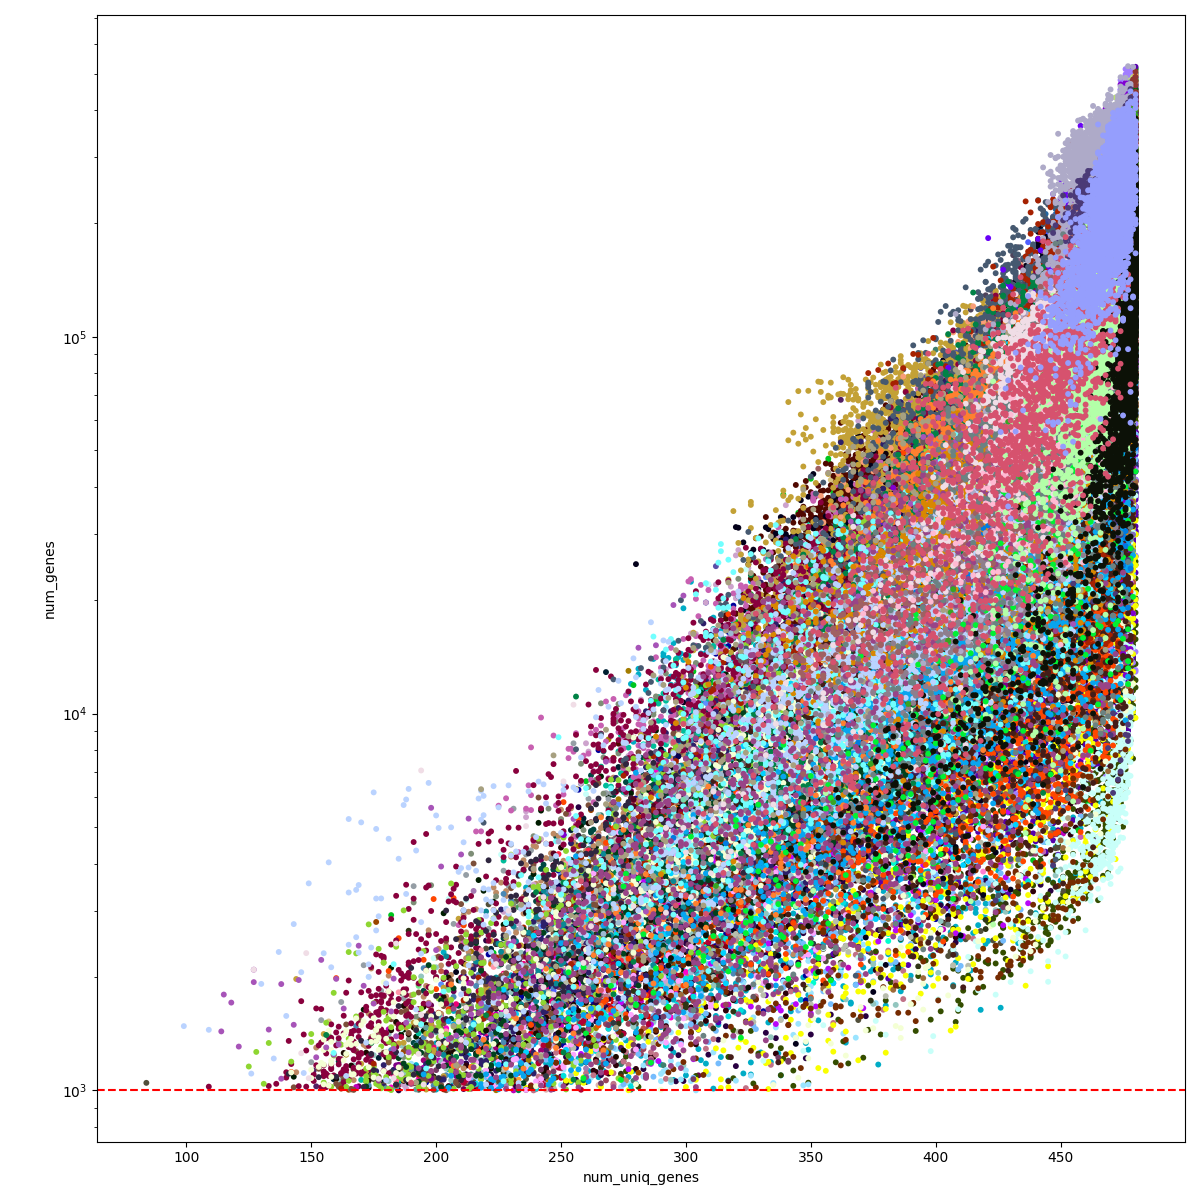
\includegraphics[width=0.8\linewidth]{figures/num_uniq_vs_num_genes_in_tiles_log.png}
  \caption{\textbf{Unique transcripts vs.\ detected genes per tile.} Relationship between the number of unique transcript molecules and the number of genes detected per tile (log scale). The strong positive correlation demonstrates that tiles with more transcripts also tend to capture more diverse gene expression, justifying our quality filtering threshold of 1,000 transcripts per tile. Points represent individual tiles across all samples.}
  \label{fig:p-fus:num-genes-tiles}
\end{figure}

\begin{figure}[t]
  \centering
  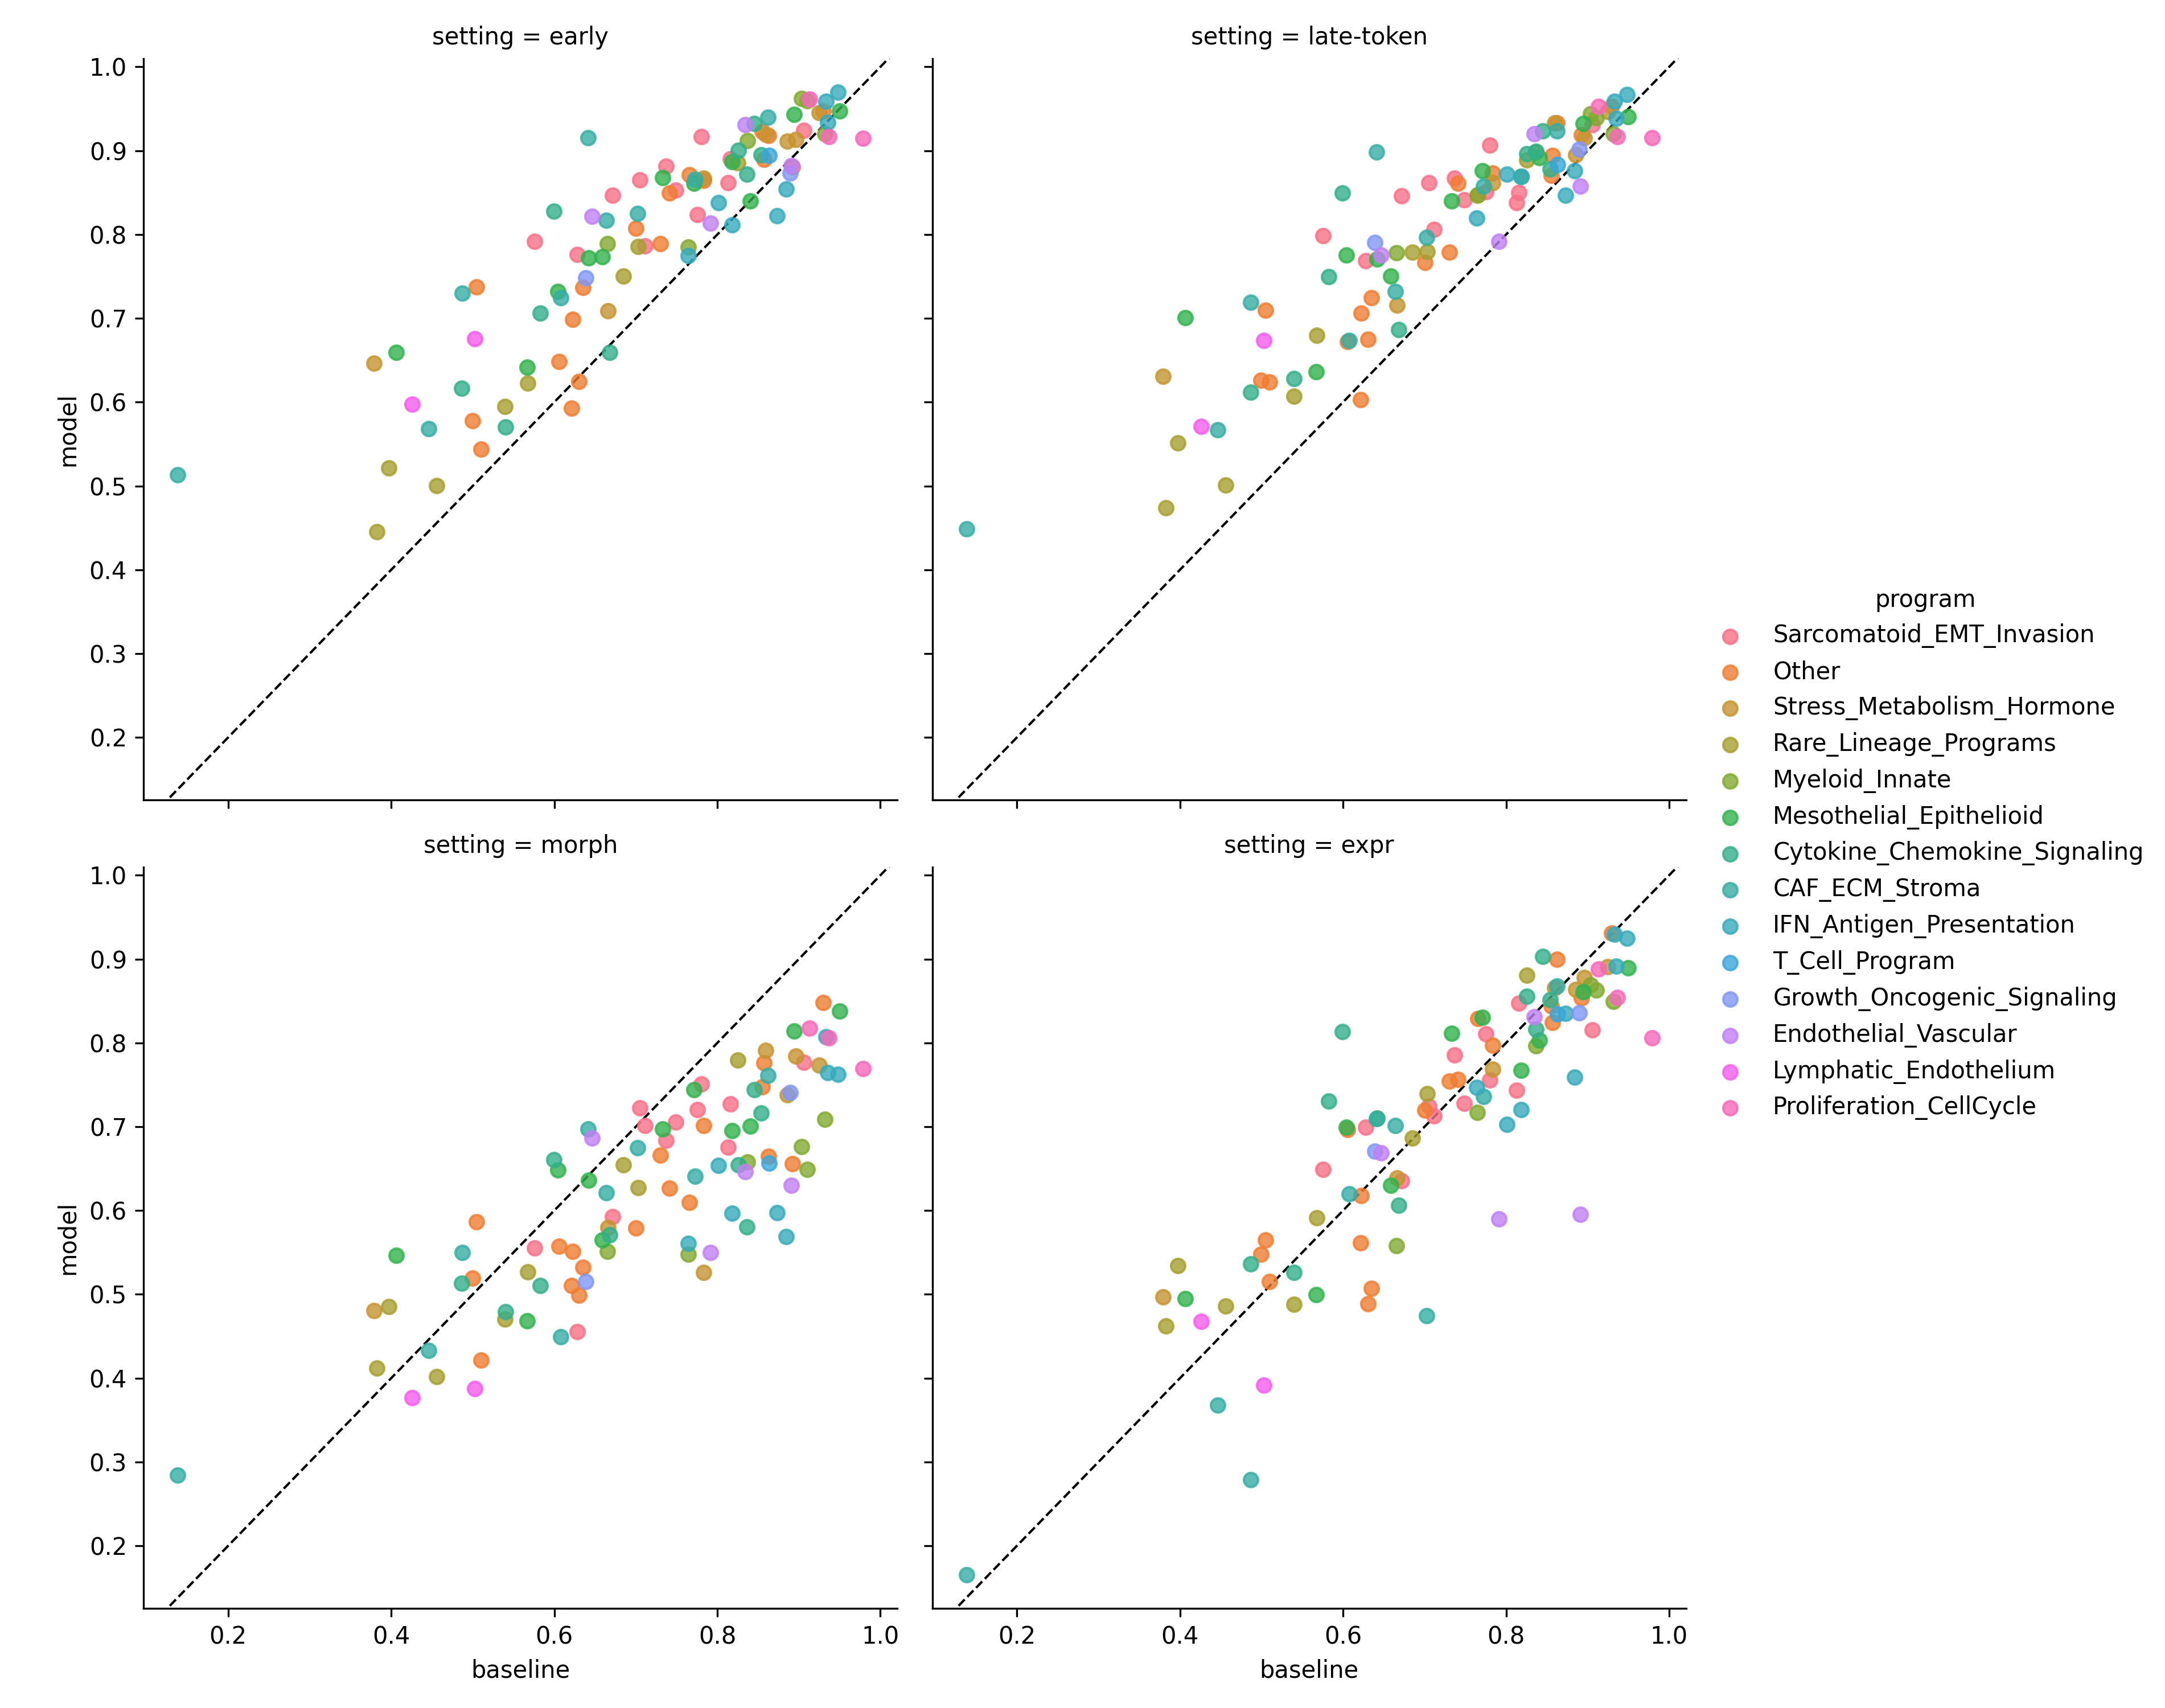
\includegraphics[width=0.95\textwidth]{figures/min_mae_predictor-scatterplot.png}
  \caption{\textbf{Comparison to Min-MAE baseline.} Spearman correlation coefficient (SCC) compared to the Min-MAE baseline for one representative split across all target genes, annotated by gene program. Both early and late fusion models substantially outperform this simple transcript-only baseline.}
  \label{fig:p-fus:main-results-minmae}
\end{figure}

%\subsection*{Model Complexity and Dataset Statistics}
%\label{sec:model-complexity-and-dataset-statistics}
%\begin{table}
  \small
  \caption{\textbf{Model complexity.} Parameter counts for all evaluated architectures, broken down by prediction head (total and trainable) and backbone (total and trainable).}
  \label{tab:p-fus:model-complexity}

\begin{tabular}{llllrrllrrrr}
\toprule
stage & strategy & morph & freeze & expr & freeze & pool & panel & \multicolumn{2}{r}{head} & \multicolumn{2}{r}{backbone} \\
 &  & encoder & morph & encoder & expr &  &  & total & trainable & total & trainable \\
\midrule
add & early & mlp & vit\_b & False & False & token & all & 30.0K & 30.0K & 86.01M & 86.01M \\
add & early & mlp & vit\_s & False & False & token & add & 15.0K & 15.0K & 21.69M & 21.69M \\
add & early & mlp & vit\_s & False & False & token & all & 15.0K & 15.0K & 21.70M & 21.70M \\
add & early & mlp & vit\_s & False & False & token & core & 15.0K & 15.0K & 21.69M & 21.69M \\
add & early & mlp & vit\_s & False & False & token & default & 38.5K & 38.5K & 21.69M & 21.69M \\
add & early & mlp & vit\_s & False & True & token & add & 15.0K & 15.0K & 21.69M & 19.9K \\
add & early & mlp & vit\_s & False & True & token & all & 15.0K & 15.0K & 21.70M & 32.1K \\
add & early & mlp & vit\_s & False & True & token & default & 38.5K & 38.5K & 21.69M & 28.9K \\
add & late & geneformer & conch & True & True & tile & - & 76.9K & 76.9K & 306.51M & 397.8K \\
add & late & geneformer & loki & True & True & tile & - & 76.9K & 76.9K & 638.85M & 397.8K \\
add & late & geneformer & midnight & True & True & tile & - & 153.7K & 153.7K & 1137.28M & 795.6K \\
add & late & geneformer & phikon & True & True & tile & - & 102.5K & 102.5K & 303.88M & 530.4K \\
add & late & geneformer & vit\_s & True & False & tile & - & 38.5K & 38.5K & 21.86M & 21.86M \\
add & late & geneformer & vit\_s & True & True & tile & - & 38.5K & 38.5K & 21.86M & 198.9K \\
add & late & mlp & conch & False & True & tile & default & 76.9K & 76.9K & 306.15M & 43.5K \\
add & late & mlp & loki & False & True & tile & - & 76.9K & 76.9K & 638.49M & 43.5K \\
add & late & mlp & phikon & False & True & tile & default & 102.5K & 102.5K & 303.41M & 53.2K \\
add & late & mlp & vit\_b & False & True & tile & all & 30.0K & 30.0K & 86.01M & 214.0K \\
add & late & mlp & vit\_b & False & True & token & all & 30.0K & 30.0K & 86.01M & 214.0K \\
add & late & mlp & vit\_s & False & False & tile & add & 15.0K & 15.0K & 21.69M & 21.69M \\
add & late & mlp & vit\_s & False & False & tile & all & 15.0K & 15.0K & 21.70M & 21.70M \\
add & late & mlp & vit\_s & False & False & tile & core & 15.0K & 15.0K & 21.69M & 21.69M \\
add & late & mlp & vit\_s & False & False & tile & default & 38.5K & 38.5K & 21.69M & 21.69M \\
add & late & mlp & vit\_s & False & False & token & add & 15.0K & 15.0K & 21.69M & 21.69M \\
add & late & mlp & vit\_s & False & False & token & all & 15.0K & 15.0K & 21.70M & 21.70M \\
add & late & mlp & vit\_s & False & False & token & core & 15.0K & 15.0K & 21.69M & 21.69M \\
add & late & mlp & vit\_s & False & False & token & default & 38.5K & 38.5K & 21.69M & 21.69M \\
add & late & mlp & vit\_s & False & True & tile & add & 15.0K & 15.0K & 21.69M & 19.9K \\
add & late & mlp & vit\_s & False & True & tile & all & 15.0K & 15.0K & 21.70M & 32.1K \\
add & late & mlp & vit\_s & False & True & tile & core & 15.0K & 15.0K & 21.69M & 28.9K \\
add & late & mlp & vit\_s & False & True & tile & default & 38.5K & 38.5K & 21.69M & 28.9K \\
add & late & mlp & vit\_s & False & True & token & add & 15.0K & 15.0K & 21.69M & 19.9K \\
add & late & mlp & vit\_s & False & True & token & all & 15.0K & 15.0K & 21.70M & 32.1K \\
add & late & mlp & vit\_s & False & True & token & core & 15.0K & 15.0K & 21.69M & 28.9K \\
add & late & mlp & vit\_s & False & True & token & default & 38.5K & 38.5K & 21.69M & 28.9K \\
concat & early & mlp & vit\_s & False & False & token & - & 38.5K & 38.5K & 21.69M & 21.69M \\
concat & late & geneformer & conch & True & True & tile & - & 153.7K & 153.7K & 306.51M & 397.8K \\
concat & late & geneformer & loki & True & True & tile & - & 153.7K & 153.7K & 638.85M & 397.8K \\
concat & late & geneformer & midnight & True & True & tile & - & 307.3K & 307.3K & 1137.28M & 795.6K \\
concat & late & geneformer & phikon & True & True & tile & - & 204.9K & 204.9K & 303.88M & 530.4K \\
concat & late & geneformer & vit\_s & True & False & tile & - & 76.9K & 76.9K & 21.86M & 21.86M \\
concat & late & geneformer & vit\_s & True & True & tile & - & 76.9K & 76.9K & 21.86M & 198.9K \\
concat & late & mlp & conch & False & True & tile & - & 153.7K & 153.7K & 306.15M & 43.5K \\
concat & late & mlp & loki & False & True & tile & - & 153.7K & 153.7K & 638.49M & 43.5K \\
concat & late & mlp & phikon & False & True & tile & - & 204.9K & 204.9K & 303.41M & 53.2K \\
concat & late & mlp & vit\_s & False & False & tile & default & 76.9K & 76.9K & 21.69M & 21.69M \\
concat & late & mlp & vit\_s & False & False & token & - & 76.9K & 76.9K & 21.69M & 21.69M \\
concat & late & mlp & vit\_s & False & True & tile & default & 76.9K & 76.9K & 21.69M & 28.9K \\
concat & late & mlp & vit\_s & False & True & token & default & 76.9K & 76.9K & 21.69M & 28.9K \\
- & - & geneformer & - & True & False & tile & - & 51.3K & 51.3K & 2.6K & 2.6K \\
- & - & mlp & - & False & False & tile & add & 1.3K & 1.3K & 5.5K & 5.5K \\
- & - & mlp & - & False & False & tile & all & 5.0K & 5.0K & 111.7K & 111.7K \\
- & - & mlp & - & False & False & tile & core & 1.3K & 1.3K & 14.5K & 14.5K \\
- & - & mlp & - & False & False & token & add & 1.3K & 1.3K & 5.5K & 5.5K \\
- & - & mlp & - & False & False & token & all & 5.0K & 5.0K & 111.7K & 111.7K \\
- & - & mlp & - & False & False & token & core & 1.3K & 1.3K & 14.5K & 14.5K \\
- & - & mlp & - & False & False & token & default & 3.3K & 3.3K & 14.5K & 14.5K \\
- & - & - & conch & False & True & token & - & 76.9K & 76.9K & 306.11M & 3.8K \\
- & - & - & loki & False & True & token & - & 76.9K & 76.9K & 638.45M & 3.8K \\
- & - & - & phikon & False & True & token & - & 102.5K & 102.5K & 303.36M & 5.1K \\
- & - & - & vit\_b & False & False & token & all & 30.0K & 30.0K & 85.80M & 85.80M \\
- & - & - & vit\_b & False & True & token & all & 30.0K & 30.0K & 85.80M & 3.8K \\
- & - & - & vit\_s & False & False & token & add & 15.0K & 15.0K & 21.67M & 21.67M \\
- & - & - & vit\_s & False & False & token & all & 15.0K & 15.0K & 21.67M & 21.67M \\
- & - & - & vit\_s & False & False & token & core & 15.0K & 15.0K & 21.67M & 21.67M \\
- & - & - & vit\_s & False & False & token & default & 38.5K & 38.5K & 21.67M & 21.67M \\
- & - & - & vit\_s & False & True & token & add & 15.0K & 15.0K & 21.67M & 1.9K \\
- & - & - & vit\_s & False & True & token & all & 15.0K & 15.0K & 21.67M & 1.9K \\
- & - & - & vit\_s & False & True & token & core & 15.0K & 15.0K & 21.67M & 1.9K \\
- & - & - & vit\_s & False & True & token & default & 38.5K & 38.5K & 21.67M & 1.9K \\
\bottomrule
\end{tabular}




\end{table}

% \begin{sidewaystable}
\begin{tabular}{lrrrrrrrrrrrrrrrrrrrrrrrrrrrrrrrrrrrrrrrr}
\toprule
Level3_grouped & B cell & CD141-positive myeloid dendritic cell & CD1c-positive myeloid dendritic cell & CD4-positive, alpha-beta T cell & CD8-positive, alpha-beta T cell & DC3 & T cell & T follicular helper cell & activated myeloid cell & adipocyte & ciliated epithelial cell & club cell & cycling lymphocyte & cycling myeloid cell & endothelial cell & endothelial cell of lymphatic vessel & fibroblast of lung & follicular dendritic cell & gamma delta T cell & germinal center B cell & heat shock myeloid cell & interferon response myeloid cell & macrophage & malignant mesothelioma cell & mast cell & mesothelial cell & monocyte & myeloid cell & nan & natural killer cell & neutrophil & pericyte & plasma cell & plasmacytoid dendritic cell & pulmonary alveolar type 1 cell & pulmonary alveolar type 2 cell & regulatory T cell & skeletal muscle fibre & type 1 interferon response T cell & unknown \\
sample_id &  &  &  &  &  &  &  &  &  &  &  &  &  &  &  &  &  &  &  &  &  &  &  &  &  &  &  &  &  &  &  &  &  &  &  &  &  &  &  &  \\
\midrule
XE_1FP2.01_HNE_1FP2-01 & 219 & 10978 & 1447 & 965 & 7615 & 1333 & 14 & 519 & 12512 & 11667 & 1192 & 342 & 5260 & 6897 & 6437 & 1968 & 25041 & 523 & 591 & 435 & 1180 & 3550 & 10654 & 73243 & 207 & 5733 & 423 & 443 & 2274 & 108 & 69 & 3023 & 253 & 73 & 174 & 34 & 1374 & 50 & 908 & 0 \\
XE_1FPK.01_HNE_1FPK-01 & 1141 & 3201 & 540 & 5319 & 30955 & 386 & 537 & 2147 & 87335 & 182 & 65 & 60 & 24073 & 5659 & 15699 & 945 & 7787 & 92 & 763 & 161 & 477 & 11846 & 2419 & 30734 & 50 & 1277 & 1813 & 589 & 184 & 635 & 147 & 15299 & 2263 & 936 & 20 & 4 & 1878 & 4 & 7009 & 0 \\
XE_1FU2.01_HNE_1FU2 & 1562 & 4183 & 3140 & 6592 & 9962 & 1056 & 173 & 893 & 6959 & 3315 & 862 & 889 & 1268 & 3850 & 26624 & 1765 & 152493 & 1956 & 1088 & 230 & 4200 & 2717 & 12195 & 57671 & 1244 & 6042 & 1172 & 1548 & 24361 & 545 & 1168 & 14189 & 8094 & 398 & 1033 & 245 & 1454 & 3632 & 1018 & 0 \\
XE_1FU3.01_HNE_1FU3-01 & 123 & 596 & 701 & 744 & 1438 & 162 & 128 & 345 & 3217 & 353 & 194 & 158 & 645 & 1360 & 1264 & 180 & 6502 & 118 & 1251 & 30 & 662 & 4576 & 3166 & 28205 & 108 & 2407 & 1030 & 137 & 529 & 158 & 606 & 1221 & 3500 & 156 & 48 & 6 & 1368 & 6 & 614 & 0 \\
XE_1FXS.01_HNE_1FXS01 & 10169 & 25643 & 14005 & 42097 & 218817 & 12280 & 10653 & 42313 & 1027600 & 18832 & 4729 & 2815 & 126029 & 148576 & 81130 & 5756 & 134361 & 12987 & 22332 & 2397 & 19935 & 79015 & 128138 & 376164 & 11748 & 72352 & 6757 & 10655 & 68915 & 2505 & 3146 & 41125 & 33179 & 5055 & 1199 & 1380 & 17114 & 396 & 26318 & 0 \\
XE_1FY2.01_HNE_1FY2 & 231066 & 14049 & 41629 & 295260 & 20688 & 7611 & 2354 & 11366 & 21000 & 27730 & 1195 & 2432 & 3551 & 11632 & 89513 & 6229 & 122951 & 36283 & 3271 & 10775 & 6330 & 4390 & 20917 & 140096 & 1594 & 25570 & 3729 & 1163 & 87450 & 2094 & 5455 & 30347 & 37206 & 13789 & 917 & 553 & 11706 & 278 & 2160 & 0 \\
XE_1FYN.01_HNE_1FYN-01 & 4143 & 10860 & 4528 & 4382 & 7941 & 4696 & 267 & 1635 & 11467 & 14946 & 19409 & 4126 & 6186 & 7143 & 37617 & 5461 & 134464 & 1540 & 1705 & 993 & 30044 & 17376 & 14953 & 287850 & 2844 & 26783 & 5026 & 2132 & 35698 & 795 & 1898 & 68523 & 4868 & 506 & 2387 & 458 & 4969 & 334 & 3456 & 0 \\
XE_1FYO.01_HNE_1FYO01 & 20514 & 15162 & 16464 & 18313 & 7041 & 2524 & 624 & 2193 & 24503 & 11943 & 3456 & 2437 & 4113 & 20939 & 34116 & 3528 & 198971 & 9041 & 1425 & 3388 & 5545 & 8263 & 20504 & 173159 & 1020 & 17703 & 2402 & 3821 & 149758 & 1036 & 1733 & 27269 & 15429 & 3293 & 3859 & 1637 & 3486 & 3015 & 1770 & 0 \\
XE_1FYS.01_HNE_1FYS & 5810 & 6566 & 6156 & 4256 & 9826 & 826 & 293 & 839 & 7955 & 5793 & 421 & 406 & 2527 & 6060 & 22514 & 3375 & 80573 & 2259 & 2412 & 1000 & 3151 & 1909 & 14966 & 89911 & 650 & 13132 & 1276 & 2732 & 40827 & 1005 & 1670 & 15690 & 23433 & 890 & 635 & 609 & 705 & 111 & 547 & 0 \\
XE_1FYT.01_HNE_1FYT & 84013 & 11820 & 11662 & 20388 & 14796 & 2065 & 1083 & 2297 & 25996 & 8880 & 1526 & 2072 & 6597 & 22677 & 54794 & 3959 & 85019 & 7234 & 12179 & 5651 & 4487 & 44459 & 17078 & 417056 & 2031 & 14653 & 3998 & 2748 & 39253 & 1705 & 632 & 19891 & 24634 & 3984 & 635 & 203 & 3024 & 230 & 7417 & 0 \\
XE_1FYV.01_HNE_1FYV-01 & 62 & 93 & 41 & 45 & 26 & 7 & 0 & 4 & 195 & 41 & 17 & 17 & 24 & 198 & 163 & 6 & 1671 & 14 & 11 & 9 & 84 & 473 & 167 & 462 & 17 & 172 & 30 & 70 & 888 & 4 & 11 & 216 & 874 & 23 & 7 & 22 & 28 & 1 & 17 & 0 \\
XE_1FZW.01_HNE_1FZW & 2096 & 14622 & 10242 & 2747 & 17493 & 2864 & 55 & 482 & 66285 & 8988 & 2431 & 1925 & 11128 & 71958 & 21973 & 4817 & 337307 & 1893 & 4006 & 1705 & 31398 & 64324 & 61424 & 171551 & 1129 & 40168 & 5835 & 5148 & 35842 & 1090 & 1963 & 30543 & 891 & 1107 & 3068 & 889 & 1498 & 263 & 4272 & 0 \\
XE_1FZX.01_HNE_1FZX01 & 5964 & 13297 & 8022 & 6844 & 7641 & 4064 & 1052 & 4043 & 59678 & 4740 & 1829 & 3092 & 7969 & 82252 & 33381 & 4142 & 238380 & 8190 & 1790 & 1180 & 35938 & 24529 & 43335 & 314473 & 1269 & 36162 & 14664 & 4181 & 32647 & 477 & 10509 & 48746 & 129917 & 1316 & 2489 & 240 & 6203 & 487 & 2662 & 0 \\
XE_1G11.01_HNE_1G11 & 44376 & 3592 & 3964 & 23136 & 7537 & 1128 & 2822 & 4172 & 9829 & 11743 & 474 & 761 & 1908 & 6186 & 28605 & 1165 & 33827 & 8861 & 2560 & 2879 & 1566 & 4484 & 17236 & 75074 & 488 & 20350 & 1193 & 971 & 33584 & 821 & 578 & 13598 & 171423 & 3306 & 239 & 376 & 1600 & 13 & 1722 & 0 \\
XE_1G11.02_HNE_1G11 & 2042 & 3078 & 2111 & 9969 & 9851 & 1195 & 1224 & 668 & 9485 & 4876 & 1338 & 879 & 1782 & 7245 & 46942 & 2641 & 121384 & 491 & 940 & 312 & 13109 & 11029 & 13674 & 46471 & 823 & 7228 & 15541 & 100880 & 28303 & 2061 & 43693 & 36694 & 3117 & 371 & 409 & 171 & 1666 & 255 & 5006 & 0 \\
XE_1G11.03_HNE_1G1103 & 19255 & 36730 & 6679 & 38712 & 314492 & 15322 & 6975 & 32641 & 707582 & 5642 & 1186 & 1650 & 145234 & 36128 & 30896 & 5048 & 174703 & 6398 & 7034 & 4088 & 14002 & 10002 & 25021 & 112661 & 396 & 27261 & 5949 & 2562 & 45890 & 2266 & 1256 & 15328 & 49485 & 8010 & 1292 & 834 & 19160 & 428 & 7352 & 0 \\
XE_1G12.01_HNE_1G12 & 8197 & 7910 & 5014 & 13548 & 3986 & 2395 & 335 & 1202 & 9449 & 8501 & 1288 & 1099 & 2390 & 3030 & 22515 & 1991 & 31559 & 4272 & 9677 & 833 & 1251 & 18494 & 6780 & 95022 & 623 & 10613 & 1336 & 1452 & 28172 & 985 & 822 & 11924 & 7697 & 2275 & 1183 & 223 & 2068 & 10286 & 5009 & 0 \\
XE_1G3S.01_HNE_1G3S-01 & 6683 & 4288 & 6260 & 14771 & 1841 & 694 & 4 & 795 & 3459 & 355 & 283 & 146 & 1063 & 13013 & 264 & 374 & 586 & 117 & 3111 & 832 & 8436 & 2354 & 11589 & 2314 & 88 & 452 & 7471 & 1070 & 12587 & 1623 & 1077 & 118 & 451 & 1608 & 75 & 55 & 1500 & 37 & 843 & 0 \\
XE_1G3U.01_HNE_1G3U & 34611 & 31304 & 16797 & 70868 & 396875 & 14077 & 7109 & 67063 & 369254 & 9023 & 6184 & 4205 & 167914 & 25361 & 71786 & 17216 & 115671 & 8598 & 18445 & 4322 & 9547 & 66802 & 52812 & 895758 & 6425 & 47649 & 10917 & 6992 & 34399 & 5154 & 2724 & 41730 & 44947 & 11680 & 1770 & 901 & 64070 & 1826 & 55354 & 0 \\
XE_1G3X.01_HNE_1G3X-01 & 2065 & 9732 & 11066 & 5679 & 7786 & 2593 & 110 & 583 & 28206 & 6373 & 2283 & 2284 & 4480 & 26447 & 39400 & 2353 & 234449 & 1184 & 2709 & 763 & 14763 & 16136 & 61403 & 472155 & 2044 & 32331 & 4723 & 2095 & 30516 & 888 & 1521 & 47965 & 1578 & 1480 & 5108 & 654 & 3583 & 418 & 2033 & 0 \\
XE_1G3Y.01_HNE_1G3Y & 11191 & 15795 & 12452 & 8508 & 6137 & 2840 & 248 & 1395 & 24401 & 11369 & 2660 & 2113 & 3056 & 16224 & 32190 & 3931 & 119841 & 4954 & 1849 & 1537 & 4695 & 9727 & 21879 & 360360 & 1615 & 32909 & 2210 & 1911 & 73124 & 574 & 645 & 21716 & 10152 & 4367 & 2884 & 1721 & 2795 & 11392 & 1844 & 0 \\
XE_1G40.01_HNE_1G40-01 & 75 & 904 & 1196 & 172 & 407 & 209 & 4 & 26 & 1058 & 589 & 691 & 397 & 359 & 4534 & 2145 & 580 & 27395 & 145 & 73 & 32 & 2546 & 890 & 2193 & 39806 & 61 & 3556 & 270 & 164 & 3264 & 24 & 39 & 2605 & 239 & 62 & 529 & 35 & 57 & 42 & 129 & 0 \\
XE_1G4J.01_HNE_1G4J-01 & 5093 & 17926 & 8094 & 17141 & 44478 & 11414 & 617 & 6186 & 105435 & 18227 & 3523 & 2391 & 16843 & 31443 & 31715 & 3424 & 269154 & 1768 & 5203 & 961 & 40386 & 34612 & 93931 & 30508 & 787 & 24972 & 31375 & 29518 & 78866 & 1324 & 2500 & 29912 & 21464 & 2373 & 2557 & 1071 & 13758 & 3427 & 6841 & 0 \\
XE_1G4K.01_HNE_1G4K & 6016 & 214 & 275 & 2679 & 428 & 88 & 40 & 621 & 375 & 537 & 70 & 37 & 83 & 50 & 3868 & 613 & 4486 & 811 & 38 & 1566 & 127 & 61 & 728 & 475 & 140 & 870 & 26 & 137 & 2635 & 58 & 55 & 1443 & 1337 & 68 & 44 & 21 & 207 & 13 & 129 & 0 \\
XE_1G4Y.01_HNE_1G4Y & 40689 & 10092 & 6277 & 12709 & 8968 & 8563 & 1056 & 4289 & 16460 & 16627 & 16936 & 5770 & 6913 & 6747 & 36925 & 4157 & 42082 & 14974 & 11886 & 7658 & 10499 & 34483 & 11133 & 146004 & 4200 & 37255 & 5415 & 4238 & 142962 & 1906 & 3331 & 15352 & 102000 & 5361 & 3304 & 1074 & 7049 & 1525 & 23605 & 0 \\
XE_1G4Z.01_HNE_1G4Z & 757 & 1302 & 1235 & 766 & 787 & 256 & 41 & 69 & 3171 & 1680 & 202 & 170 & 317 & 1112 & 13327 & 1895 & 15205 & 720 & 835 & 139 & 374 & 2813 & 1864 & 22191 & 397 & 3587 & 780 & 962 & 7691 & 656 & 832 & 5849 & 3433 & 298 & 267 & 37 & 132 & 6268 & 468 & 0 \\
XE_1G50.01_HNE_1G50 & 1686 & 4019 & 8970 & 7955 & 11900 & 1166 & 252 & 1469 & 11362 & 3977 & 584 & 1043 & 2989 & 13579 & 14337 & 2284 & 91572 & 1512 & 2809 & 254 & 6423 & 5689 & 26794 & 135319 & 471 & 8874 & 2311 & 1170 & 8746 & 815 & 481 & 8907 & 1121 & 620 & 437 & 246 & 4529 & 222 & 2997 & 0 \\
XE_1G51.01_HNE_1G51 & 39455 & 20924 & 23673 & 16438 & 14879 & 6654 & 1405 & 3599 & 30113 & 10467 & 2198 & 3611 & 9652 & 51119 & 29132 & 4618 & 69223 & 23279 & 6714 & 11316 & 10110 & 33125 & 41909 & 197741 & 1299 & 41108 & 5292 & 4225 & 135207 & 2240 & 15895 & 15209 & 55743 & 5804 & 839 & 596 & 4358 & 149 & 7471 & 0 \\
XE_1G5A.01_HNE_1G5A & 297 & 3603 & 1448 & 1528 & 5054 & 1350 & 18 & 1141 & 14713 & 2552 & 4430 & 1086 & 4742 & 6577 & 10407 & 2866 & 171968 & 777 & 500 & 484 & 10986 & 5617 & 11311 & 141605 & 819 & 13785 & 2109 & 1099 & 28893 & 177 & 430 & 22796 & 1459 & 206 & 2412 & 501 & 1469 & 2654 & 1539 & 0 \\
XE_1G5A.02_HNE_1G5A & 480428 & 67002 & 21449 & 350612 & 25685 & 44035 & 4217 & 27504 & 41780 & 23196 & 5692 & 6646 & 18381 & 5056 & 161281 & 248521 & 55095 & 173775 & 12949 & 56478 & 2710 & 7741 & 15333 & 112296 & 5240 & 29977 & 6529 & 5496 & 387804 & 5681 & 3887 & 74922 & 318454 & 41351 & 1499 & 769 & 28474 & 1047 & 13697 & 0 \\
XE_1G5B.01_HNE_1G5B-01 & 5342 & 3116 & 2997 & 4600 & 3237 & 668 & 335 & 495 & 4848 & 6089 & 733 & 738 & 835 & 1403 & 25077 & 1595 & 49476 & 1828 & 602 & 506 & 1513 & 920 & 6688 & 19628 & 336 & 6398 & 552 & 1922 & 27039 & 722 & 1283 & 13384 & 12033 & 426 & 400 & 108 & 469 & 59 & 142 & 0 \\
XE_1G63.01_HNE_1G63-01 & 1028 & 1865 & 2145 & 2216 & 9626 & 766 & 448 & 1020 & 13243 & 2094 & 302 & 366 & 5020 & 5719 & 8810 & 1276 & 24814 & 1181 & 4004 & 183 & 683 & 5768 & 8869 & 65525 & 507 & 8959 & 1117 & 481 & 7021 & 637 & 1418 & 7288 & 13260 & 469 & 325 & 189 & 1662 & 14516 & 834 & 0 \\
XE_1G6Z.01_HNE_1G6Z-01 & 1064 & 720 & 769 & 443 & 363 & 161 & 3 & 58 & 1026 & 480 & 102 & 89 & 104 & 1086 & 3900 & 609 & 11880 & 80 & 706 & 82 & 347 & 602 & 2886 & 36760 & 272 & 1950 & 192 & 355 & 3482 & 130 & 287 & 1824 & 308 & 37 & 102 & 75 & 110 & 605 & 98 & 0 \\
XE_1G96.01_HNE_1G96 & 13743 & 10778 & 11587 & 21642 & 34751 & 6542 & 3350 & 6773 & 51086 & 7436 & 1848 & 1969 & 10574 & 22830 & 21323 & 1690 & 385031 & 4108 & 11437 & 1337 & 6598 & 5692 & 56244 & 80631 & 1094 & 57530 & 3943 & 2078 & 49610 & 1600 & 510 & 15763 & 115275 & 1043 & 1344 & 617 & 10746 & 180 & 3296 & 0 \\
XE_1G97.01_HNE_1G97-01 & 205 & 1062 & 1034 & 517 & 302 & 302 & 4 & 38 & 2981 & 1614 & 1530 & 411 & 1071 & 3089 & 4114 & 1900 & 38537 & 159 & 170 & 77 & 12923 & 1679 & 4879 & 19564 & 237 & 3653 & 1173 & 1584 & 10066 & 109 & 418 & 4655 & 102 & 147 & 595 & 109 & 201 & 1508 & 1050 & 0 \\
XE_1G9C.01_HNE_1G9C & 95814 & 18708 & 66365 & 164796 & 47406 & 7518 & 8165 & 9154 & 49118 & 19542 & 2454 & 4590 & 8692 & 14678 & 69535 & 5026 & 297353 & 26132 & 4200 & 4869 & 5252 & 15944 & 42157 & 335018 & 2217 & 56873 & 6226 & 2228 & 40846 & 3250 & 1014 & 29502 & 63699 & 15880 & 1246 & 660 & 9747 & 190 & 12144 & 0 \\
XE_1GB9.01_HNE_1GB9 & 2012 & 5776 & 5377 & 10906 & 22343 & 1685 & 778 & 1958 & 12062 & 9057 & 569 & 781 & 2775 & 9127 & 31011 & 2012 & 262558 & 1295 & 1527 & 120 & 1523 & 6497 & 29132 & 65981 & 1025 & 10275 & 2896 & 1036 & 14269 & 792 & 3097 & 20212 & 11602 & 1417 & 446 & 319 & 4619 & 82 & 1558 & 0 \\
XE_1GBF.01_HNE_1GBF-01 & 940 & 1424 & 1624 & 3028 & 2370 & 389 & 53 & 251 & 6861 & 793 & 183 & 108 & 1289 & 9086 & 6566 & 487 & 27955 & 260 & 4051 & 103 & 698 & 9029 & 26281 & 112112 & 414 & 7457 & 1126 & 362 & 911 & 237 & 1412 & 4534 & 572 & 161 & 79 & 46 & 702 & 12 & 1110 & 0 \\
XE_1GCY.01_HNE_1GCY & 55928 & 7379 & 13305 & 45901 & 53731 & 3201 & 3618 & 10018 & 48189 & 2560 & 382 & 458 & 13298 & 16691 & 27100 & 3994 & 77023 & 8184 & 4461 & 13344 & 4032 & 6246 & 33977 & 232764 & 5138 & 17086 & 6237 & 1939 & 10335 & 1663 & 332 & 17228 & 60152 & 3262 & 285 & 190 & 14438 & 73 & 1605 & 0 \\
XE_1GEG.01_HNE_1GEG & 91126 & 14325 & 11598 & 35789 & 45288 & 6432 & 4881 & 12804 & 75693 & 6560 & 1368 & 1075 & 12954 & 14994 & 35785 & 18723 & 184307 & 5863 & 6306 & 15619 & 10887 & 11222 & 24664 & 84084 & 750 & 28203 & 9029 & 4004 & 87622 & 2702 & 1788 & 41374 & 336301 & 2807 & 770 & 672 & 10900 & 116 & 5548 & 0 \\
XE_1GEM.01_HNE_1GEM-01 & 187 & 829 & 738 & 273 & 138 & 480 & 15 & 18 & 831 & 720 & 935 & 445 & 293 & 2335 & 944 & 719 & 12540 & 108 & 110 & 97 & 2637 & 706 & 2319 & 38416 & 217 & 3726 & 460 & 1364 & 3164 & 5 & 193 & 662 & 67 & 64 & 854 & 35 & 82 & 47 & 26 & 0 \\
XE_1GEP.01_HNE_1GEP & 10724 & 29803 & 5828 & 39514 & 383859 & 21810 & 5907 & 37978 & 598562 & 2208 & 578 & 540 & 167638 & 26098 & 34429 & 375 & 179945 & 1185 & 9318 & 3157 & 5615 & 6207 & 16011 & 21785 & 141 & 19559 & 7711 & 1260 & 7927 & 3335 & 1201 & 20732 & 33150 & 15204 & 331 & 233 & 18840 & 74 & 7534 & 0 \\
XE_1GGF.01_HNE_1GGF & 3258 & 6206 & 11513 & 12657 & 18875 & 3573 & 1363 & 4668 & 18253 & 6718 & 2133 & 1319 & 4859 & 23145 & 37589 & 2603 & 452075 & 3757 & 1464 & 448 & 10888 & 7359 & 61444 & 14562 & 1204 & 17989 & 6218 & 5077 & 18568 & 652 & 1874 & 24120 & 18232 & 1124 & 735 & 327 & 7207 & 2251 & 4500 & 0 \\
XE_1GGR.01_HNE_1GGR & 15909 & 50054 & 26833 & 27100 & 69008 & 7204 & 2128 & 11545 & 138588 & 25914 & 5799 & 13063 & 34747 & 49815 & 61597 & 6000 & 422950 & 8659 & 29356 & 3100 & 16832 & 93836 & 89556 & 722512 & 2772 & 124643 & 11582 & 9211 & 152984 & 2939 & 1446 & 50859 & 27808 & 4859 & 7726 & 3578 & 8720 & 17201 & 13531 & 0 \\
XE_1GJB.01_HNE_1GJB & 4474 & 3837 & 2937 & 8008 & 5263 & 1341 & 126 & 2051 & 7732 & 2939 & 307 & 311 & 2163 & 3075 & 9102 & 397 & 9307 & 1155 & 1188 & 380 & 748 & 11771 & 6024 & 53151 & 154 & 2086 & 848 & 839 & 11047 & 353 & 363 & 2764 & 3315 & 1197 & 215 & 93 & 2925 & 217 & 12812 & 0 \\
XE_1GJC.01_HNE_1GJC & 421599 & 12009 & 14876 & 90064 & 16599 & 2425 & 5035 & 6535 & 41159 & 17255 & 1489 & 1475 & 4406 & 49091 & 65570 & 2469 & 239694 & 42080 & 6359 & 10795 & 5798 & 57196 & 31950 & 686566 & 2494 & 60772 & 7037 & 2820 & 14751 & 1526 & 1674 & 34720 & 75142 & 15556 & 903 & 480 & 6204 & 126 & 5099 & 0 \\
XE_1GK0.01_HNE_1GK0 & 5399 & 21384 & 13937 & 15262 & 38169 & 3692 & 1234 & 5771 & 42462 & 12751 & 3270 & 3921 & 15666 & 41019 & 36213 & 3575 & 177682 & 4071 & 18371 & 1008 & 7618 & 15982 & 38137 & 730531 & 4792 & 60906 & 4871 & 1572 & 73753 & 2353 & 836 & 33670 & 57533 & 2554 & 7259 & 2786 & 4585 & 332 & 6536 & 0 \\
XE_1GNX.01_HNE_1GNX & 12670 & 13198 & 11611 & 8670 & 2999 & 3082 & 296 & 1277 & 8189 & 7427 & 6657 & 3552 & 3375 & 9237 & 23386 & 4123 & 237882 & 5333 & 1321 & 2284 & 4576 & 3642 & 7903 & 201077 & 1426 & 34392 & 2455 & 1522 & 95934 & 605 & 729 & 21772 & 33329 & 789 & 4780 & 840 & 1550 & 659 & 686 & 0 \\
XE_1GP1.01_HNE_1GP1 & 37306 & 12176 & 19785 & 55525 & 160560 & 7737 & 20330 & 15982 & 177803 & 15460 & 2017 & 1624 & 48889 & 39426 & 51638 & 1600 & 155642 & 6660 & 54561 & 4727 & 18409 & 19067 & 100308 & 781187 & 3306 & 37176 & 29566 & 5800 & 53120 & 5192 & 4893 & 29829 & 217743 & 3422 & 703 & 485 & 28073 & 334 & 9355 & 0 \\
XE_1GPD.01_HNE_1GPD & 6627 & 976 & 2713 & 7065 & 2316 & 403 & 235 & 1240 & 2400 & 1046 & 141 & 73 & 524 & 1929 & 6561 & 308 & 16333 & 2489 & 286 & 1744 & 420 & 3103 & 4542 & 6265 & 112 & 4331 & 733 & 105 & 2832 & 123 & 137 & 3156 & 12030 & 694 & 39 & 24 & 619 & 9 & 555 & 0 \\
XE_1GPO.01_HNE_1GPO & 1031 & 7365 & 14555 & 5367 & 25357 & 972 & 2664 & 2638 & 50248 & 2252 & 572 & 749 & 11017 & 36144 & 18457 & 785 & 37038 & 2439 & 5520 & 197 & 2293 & 61618 & 43204 & 178347 & 293 & 18685 & 2174 & 991 & 13200 & 649 & 992 & 12662 & 16970 & 486 & 701 & 240 & 11554 & 104 & 6207 & 0 \\
XE_1GPP.01_HNE_1GPP-01 & 3787 & 14391 & 17929 & 20361 & 88535 & 4769 & 544 & 6661 & 184258 & 7076 & 3068 & 4541 & 42424 & 123361 & 43574 & 2180 & 86500 & 2101 & 7464 & 1287 & 54185 & 92251 & 95976 & 858424 & 1804 & 24529 & 18157 & 4795 & 75932 & 2049 & 6359 & 44400 & 1717 & 4198 & 2535 & 606 & 14651 & 771 & 24312 & 0 \\
XE_1GPT.01_HNE_1GPT & 25910 & 11019 & 11697 & 33126 & 18824 & 4573 & 379 & 6714 & 67157 & 6933 & 1475 & 1665 & 15212 & 34650 & 54253 & 6396 & 168435 & 5530 & 5999 & 1637 & 8651 & 26872 & 59684 & 162769 & 846 & 20979 & 8678 & 3829 & 13480 & 1707 & 2156 & 28809 & 4379 & 3016 & 832 & 445 & 16461 & 105 & 8559 & 0 \\
XE_1GPZ.01_HNE_1GPZ & 14149 & 4896 & 2382 & 8505 & 1511 & 1928 & 261 & 1206 & 8119 & 4388 & 1116 & 1259 & 1532 & 3440 & 16662 & 1058 & 12861 & 4776 & 3561 & 1752 & 1114 & 24932 & 8507 & 148655 & 728 & 18777 & 2622 & 1655 & 53735 & 595 & 1895 & 6634 & 18924 & 2352 & 434 & 130 & 1024 & 249 & 3339 & 0 \\
XE_1GQ8.01_HNE_1GQ8 & 16882 & 5883 & 18386 & 13233 & 13120 & 3467 & 4047 & 4387 & 16322 & 17003 & 797 & 745 & 4514 & 19437 & 35220 & 1172 & 249680 & 7148 & 1665 & 1137 & 3955 & 3805 & 26780 & 161078 & 812 & 25524 & 3584 & 1058 & 20213 & 619 & 438 & 24373 & 197404 & 975 & 383 & 162 & 8530 & 30 & 1237 & 0 \\
XE_1GQR.01_HNE_1GQR & 76324 & 13731 & 22679 & 48370 & 10139 & 2339 & 1501 & 3481 & 19555 & 16053 & 1053 & 2163 & 2561 & 12216 & 48167 & 4053 & 177494 & 13815 & 2124 & 7140 & 3547 & 5332 & 33055 & 56111 & 1096 & 18655 & 2908 & 3306 & 38202 & 1580 & 911 & 25939 & 89544 & 6039 & 596 & 686 & 2954 & 62 & 844 & 0 \\
XE_1GS0.01_HNE_1GS0-01 & 7056 & 5980 & 17199 & 14394 & 16552 & 1502 & 1264 & 1215 & 7834 & 2034 & 690 & 692 & 3557 & 69419 & 33526 & 925 & 132143 & 1163 & 10791 & 607 & 1345 & 32658 & 34257 & 443801 & 772 & 14447 & 14082 & 480 & 5652 & 796 & 1345 & 34332 & 26098 & 1194 & 428 & 88 & 2580 & 32 & 4587 & 0 \\
XE_1GS6.01_HNE_1GS6 & 88024 & 12638 & 6157 & 107951 & 37643 & 15029 & 11851 & 38513 & 68988 & 3766 & 1013 & 1448 & 20798 & 9479 & 32152 & 19965 & 13479 & 20126 & 3921 & 33229 & 7696 & 4188 & 19025 & 222249 & 383 & 13204 & 5725 & 1414 & 76712 & 2671 & 3312 & 9670 & 431403 & 7510 & 740 & 470 & 23717 & 57 & 3066 & 0 \\
XE_1GTE.01_HNE_1GTE-01 & 113030 & 29512 & 30886 & 152924 & 89703 & 9397 & 26607 & 17269 & 41168 & 24777 & 2973 & 2919 & 24656 & 53936 & 126605 & 14127 & 149037 & 14214 & 18440 & 5703 & 6753 & 42466 & 91433 & 668730 & 3992 & 161398 & 14059 & 3355 & 43062 & 3255 & 3783 & 103868 & 354778 & 7546 & 1765 & 1680 & 10190 & 1734 & 20623 & 0 \\
XE_1GTK.01_HNE_1GTK-01 & 4691 & 685 & 527 & 2120 & 2464 & 428 & 81 & 591 & 1061 & 3629 & 320 & 371 & 391 & 440 & 12320 & 384 & 10906 & 1249 & 400 & 632 & 224 & 1308 & 2184 & 1949 & 215 & 2501 & 153 & 265 & 11607 & 492 & 94 & 3954 & 8389 & 229 & 79 & 38 & 200 & 68 & 1273 & 0 \\
XE_1GUG.01_HNE_1GUG & 43700 & 10388 & 9183 & 47157 & 19390 & 5940 & 1369 & 13291 & 37214 & 9113 & 2443 & 992 & 7653 & 6941 & 18331 & 3150 & 25053 & 15961 & 2064 & 6777 & 3124 & 6601 & 12024 & 10119 & 1093 & 7233 & 4774 & 5576 & 78650 & 1630 & 1681 & 9515 & 67952 & 4856 & 717 & 296 & 7814 & 272 & 6598 & 0 \\
XE_1GV3.01_HNE_1GV3 & 4939 & 4337 & 6506 & 7918 & 9388 & 1243 & 1234 & 2392 & 12517 & 5867 & 908 & 608 & 2693 & 37873 & 24609 & 1497 & 88813 & 3186 & 2539 & 728 & 5730 & 9411 & 42614 & 176902 & 878 & 18648 & 1729 & 2881 & 15947 & 769 & 2124 & 12463 & 20441 & 754 & 220 & 234 & 1400 & 82 & 2858 & 0 \\
XE_1GVN.01_HNE_1GVN & 2014 & 12038 & 10435 & 9166 & 14576 & 2916 & 849 & 1817 & 53192 & 5386 & 1184 & 1492 & 5102 & 95756 & 30773 & 2800 & 123113 & 2214 & 59221 & 567 & 28506 & 26158 & 148345 & 1355238 & 3284 & 9695 & 4311 & 2635 & 5738 & 1231 & 2851 & 27267 & 8790 & 902 & 2061 & 1029 & 5127 & 354 & 3649 & 0 \\
XE_1GVX.01_HNE_1GVX-01 & 1977 & 18675 & 11795 & 14663 & 23428 & 3136 & 445 & 3131 & 77600 & 7313 & 1079 & 1114 & 9290 & 24228 & 24582 & 1346 & 135789 & 1665 & 9029 & 610 & 3201 & 12948 & 39822 & 160423 & 540 & 27097 & 4017 & 2607 & 52247 & 1797 & 4561 & 16182 & 1636 & 951 & 1438 & 913 & 4977 & 74 & 5034 & 0 \\
XE_1GWV.01_HNE_1GWV & 49568 & 6041 & 20151 & 30831 & 4018 & 1786 & 472 & 2844 & 8866 & 11082 & 482 & 856 & 961 & 4903 & 32815 & 1352 & 86704 & 8092 & 1259 & 1839 & 1480 & 1977 & 17548 & 88030 & 1522 & 5326 & 2726 & 1153 & 14080 & 534 & 441 & 16426 & 20163 & 4608 & 441 & 140 & 2133 & 16171 & 788 & 0 \\
XE_1GX4.01_HNE_1GX4-01 & 0 & 0 & 0 & 1 & 0 & 1 & 0 & 0 & 0 & 2 & 1 & 2 & 0 & 4 & 1 & 0 & 16 & 1 & 1 & 0 & 6 & 0 & 3 & 10 & 0 & 2 & 0 & 0 & 46 & 0 & 0 & 1 & 0 & 0 & 5 & 0 & 1 & 1 & 1 & 0 \\
XE_1GXI.01_HNE_1GXI-01 & 6598 & 11353 & 27318 & 27386 & 14288 & 3172 & 1568 & 1143 & 103786 & 9661 & 2895 & 6163 & 4565 & 68960 & 62346 & 4603 & 117966 & 1603 & 25602 & 1067 & 24879 & 135716 & 193890 & 962067 & 824 & 33082 & 35696 & 6371 & 11540 & 1446 & 1409 & 39115 & 3704 & 1328 & 935 & 406 & 4111 & 482 & 10579 & 0 \\
XE_1GY0.01_HNE_1GY0 & 21767 & 19826 & 16824 & 25410 & 12755 & 5565 & 551 & 2379 & 33130 & 5468 & 2022 & 3448 & 5170 & 23201 & 34787 & 8274 & 236480 & 4176 & 2492 & 3893 & 11505 & 11556 & 37777 & 114119 & 826 & 17175 & 4726 & 3675 & 84543 & 1340 & 1839 & 36560 & 16487 & 2120 & 966 & 587 & 5174 & 311 & 2637 & 0 \\
XE_1GY1.01_HNE_1GY1-01 & 1840 & 1609 & 973 & 444 & 540 & 425 & 42 & 130 & 3116 & 1015 & 769 & 769 & 594 & 3579 & 5426 & 385 & 11929 & 773 & 904 & 236 & 2320 & 9715 & 2593 & 135996 & 189 & 3491 & 599 & 512 & 9086 & 157 & 274 & 4828 & 7192 & 249 & 392 & 27 & 309 & 3354 & 1632 & 0 \\
XE_1GY3.01_HNE_1GY3-01 & 279 & 3355 & 2811 & 1382 & 3197 & 862 & 0 & 355 & 7967 & 4955 & 1164 & 1118 & 2114 & 15583 & 8192 & 606 & 9538 & 759 & 3656 & 213 & 3035 & 2653 & 23530 & 203708 & 246 & 11464 & 764 & 485 & 36709 & 188 & 110 & 20346 & 19 & 162 & 1606 & 299 & 790 & 80 & 591 & 0 \\
XE_1H0S.01_HNE_1H0S-01 & 31427 & 3553 & 3446 & 19878 & 5410 & 992 & 769 & 3582 & 5781 & 5560 & 379 & 380 & 941 & 1875 & 17939 & 2211 & 36392 & 9380 & 892 & 2471 & 1742 & 1265 & 14969 & 10522 & 531 & 5543 & 963 & 1716 & 20999 & 684 & 303 & 7214 & 47031 & 1092 & 301 & 285 & 1920 & 53 & 276 & 0 \\
XE_1H0T.01_HNE_1H0T & 831 & 2127 & 2517 & 2443 & 3012 & 747 & 299 & 672 & 8054 & 884 & 628 & 1091 & 1198 & 3910 & 4240 & 510 & 16847 & 260 & 6783 & 83 & 482 & 31786 & 13773 & 117748 & 717 & 7305 & 1478 & 942 & 14928 & 188 & 97 & 3388 & 5111 & 1032 & 334 & 83 & 2315 & 104 & 5485 & 0 \\
XE_1H20.01_HNE_1H20_01 & 16170 & 19629 & 22358 & 28594 & 29057 & 5898 & 1467 & 5176 & 52016 & 15222 & 3988 & 4231 & 10107 & 108894 & 86843 & 9145 & 414136 & 11803 & 4749 & 1212 & 20669 & 34207 & 108613 & 648541 & 2568 & 58404 & 6370 & 5301 & 52390 & 1678 & 1620 & 61030 & 41114 & 6426 & 2348 & 1371 & 11980 & 11401 & 12707 & 0 \\
XE_1H3W.01_HNE_1H3W_01 & 305 & 1136 & 2218 & 2329 & 2395 & 324 & 7 & 275 & 10841 & 198 & 74 & 45 & 806 & 6254 & 83 & 139 & 194 & 48 & 2956 & 45 & 17918 & 150505 & 1218 & 8352 & 46 & 44 & 2028 & 205 & 1871 & 78 & 681 & 63 & 1517 & 2929 & 44 & 4 & 1173 & 28 & 2193 & 0 \\
XE_1H49.01_HNE_1H49_01_-_5 & 6916 & 4533 & 4097 & 11147 & 14583 & 1853 & 626 & 2211 & 8273 & 6614 & 1088 & 1429 & 2617 & 929 & 58853 & 10201 & 80219 & 2272 & 2629 & 1303 & 3409 & 1259 & 7583 & 1653 & 1257 & 13059 & 689 & 2928 & 28208 & 2065 & 327 & 31744 & 25750 & 595 & 1037 & 734 & 2474 & 239 & 1655 & 0 \\
XE_1H49.03_HNE_1H49_03_-_7 & 2387 & 4991 & 4114 & 6712 & 34172 & 2482 & 2773 & 2999 & 66837 & 3472 & 579 & 414 & 9180 & 3776 & 26104 & 4015 & 35516 & 1715 & 4748 & 514 & 2056 & 5845 & 10109 & 54356 & 601 & 16910 & 1475 & 3956 & 56482 & 1811 & 306 & 11285 & 116902 & 937 & 373 & 548 & 4415 & 319 & 4529 & 0 \\
XE_1H49.04_HNE_1H49-04 & 2658 & 15058 & 4952 & 16412 & 129854 & 3615 & 6795 & 9418 & 162441 & 4675 & 923 & 551 & 22065 & 4447 & 32089 & 6850 & 133060 & 952 & 6806 & 513 & 3794 & 15570 & 11855 & 32413 & 466 & 15174 & 4092 & 4244 & 47050 & 3200 & 1621 & 24964 & 80613 & 3355 & 370 & 980 & 9288 & 2275 & 11641 & 0 \\
XE_1H4A.01_HNE_1H4A & 581 & 4521 & 5507 & 1550 & 2555 & 844 & 4 & 370 & 20255 & 1798 & 645 & 819 & 1402 & 17755 & 14043 & 849 & 64122 & 350 & 493 & 228 & 18881 & 9451 & 32485 & 57194 & 538 & 6117 & 8960 & 7091 & 50176 & 603 & 4919 & 15532 & 628 & 521 & 873 & 246 & 1683 & 225 & 443 & 0 \\
XE_1H4D.01_HNE_1H4D & 56007 & 5722 & 12672 & 29339 & 13355 & 2144 & 1647 & 6084 & 14420 & 12338 & 888 & 708 & 4391 & 15228 & 39801 & 5129 & 105039 & 16633 & 3468 & 4849 & 3215 & 7082 & 42885 & 160983 & 2260 & 22631 & 2827 & 2360 & 18572 & 944 & 1846 & 24099 & 25341 & 3891 & 542 & 189 & 3379 & 20904 & 2823 & 0 \\
XE_1H4E.01_HNE_1H4E-01 & 33946 & 2392 & 2300 & 19180 & 2922 & 781 & 609 & 2156 & 6258 & 1453 & 379 & 367 & 559 & 2945 & 10872 & 1031 & 21095 & 7479 & 701 & 5079 & 1635 & 1757 & 13981 & 30925 & 459 & 18821 & 1593 & 1782 & 20586 & 310 & 953 & 6329 & 41911 & 1435 & 191 & 130 & 1136 & 46 & 374 & 0 \\
XE_1H50.01_HNE_1H50-01 & 68784 & 4323 & 6356 & 48619 & 15997 & 1600 & 1687 & 6412 & 13793 & 8723 & 801 & 551 & 1777 & 2379 & 22503 & 1349 & 34424 & 12130 & 2427 & 4363 & 1505 & 12253 & 11157 & 9127 & 706 & 15028 & 1552 & 732 & 12380 & 794 & 200 & 13058 & 11272 & 1968 & 311 & 189 & 2945 & 34 & 2623 & 0 \\
XE_1H5I.01_HNE_1H5I & 2249 & 13556 & 6669 & 5337 & 6740 & 2877 & 225 & 1083 & 20406 & 5872 & 2532 & 3290 & 5047 & 95474 & 25547 & 3648 & 355756 & 3196 & 21030 & 812 & 22614 & 8636 & 49320 & 1288682 & 1641 & 35447 & 3450 & 1590 & 62179 & 1202 & 898 & 19735 & 1983 & 608 & 2545 & 834 & 2262 & 414 & 4355 & 0 \\
XE_1H5M.01_HNE_1H5M-01 & 45551 & 10758 & 9923 & 29982 & 14106 & 3733 & 632 & 3835 & 37542 & 6941 & 2210 & 2050 & 7693 & 39626 & 75688 & 3753 & 828563 & 4699 & 1865 & 1349 & 9919 & 12829 & 61787 & 8151 & 2619 & 22712 & 4914 & 5315 & 52668 & 1504 & 1300 & 49924 & 23503 & 1796 & 1427 & 779 & 6330 & 177 & 3156 & 0 \\
XE_1HDD.01_HNE_1HDD & 11117 & 665 & 1467 & 4486 & 1067 & 172 & 124 & 868 & 1232 & 1673 & 209 & 279 & 217 & 389 & 11395 & 1727 & 16500 & 863 & 135 & 3914 & 348 & 570 & 3371 & 1405 & 271 & 2895 & 132 & 393 & 5259 & 145 & 251 & 5072 & 7398 & 117 & 93 & 36 & 546 & 19 & 57 & 0 \\
XE_1HFS.01_HNE_1HFS & 17682 & 8377 & 9264 & 12717 & 4838 & 1836 & 698 & 1328 & 10437 & 4276 & 2896 & 1064 & 2573 & 31837 & 20370 & 3628 & 187652 & 4728 & 901 & 1963 & 4659 & 7662 & 29169 & 167333 & 516 & 17065 & 2382 & 1184 & 27239 & 262 & 508 & 25771 & 10650 & 653 & 780 & 229 & 2277 & 144 & 994 & 0 \\
XE_1HHP.0B_HNE_1HHP-0B & 917 & 8089 & 8075 & 6985 & 38007 & 1832 & 402 & 1732 & 33468 & 3125 & 437 & 287 & 11777 & 32627 & 11473 & 1206 & 117728 & 445 & 17967 & 336 & 10780 & 6672 & 75084 & 429308 & 308 & 17510 & 5334 & 2328 & 3433 & 1243 & 332 & 11856 & 5628 & 480 & 338 & 104 & 5110 & 130 & 3542 & 0 \\
XE_1HHR.01_HNE_1HHR-01 & 969 & 1357 & 8481 & 2823 & 2468 & 1039 & 29 & 449 & 11971 & 1592 & 365 & 194 & 1997 & 7398 & 13367 & 1294 & 94345 & 728 & 779 & 187 & 10382 & 4471 & 14209 & 449795 & 1306 & 47765 & 26592 & 1161 & 2525 & 135 & 519 & 14891 & 783 & 648 & 161 & 39 & 2183 & 99 & 820 & 0 \\
XE_1HJ3.01_HNE_1HJ3-01 & 25844 & 5140 & 7568 & 31040 & 7291 & 1928 & 1329 & 3162 & 7650 & 8171 & 1376 & 1030 & 1691 & 4211 & 51020 & 6423 & 93921 & 8986 & 1075 & 2196 & 3012 & 2933 & 15096 & 22214 & 1570 & 11847 & 3547 & 1451 & 46806 & 990 & 5769 & 29916 & 85481 & 1099 & 388 & 283 & 3004 & 2054 & 2033 & 0 \\
XE_1HJ6.01_HNE_1HJ6-01 & 45463 & 9153 & 3901 & 45972 & 22783 & 3015 & 1627 & 5036 & 19872 & 6741 & 1751 & 1457 & 8179 & 5831 & 49299 & 1577 & 63210 & 4016 & 23650 & 4948 & 4010 & 54394 & 29618 & 770959 & 1299 & 60677 & 4381 & 1000 & 25175 & 2962 & 1004 & 30175 & 27981 & 2714 & 679 & 215 & 10580 & 292 & 15982 & 0 \\
XE_1HJ7.01_HNE_1HJ7 & 2935 & 6265 & 4085 & 5085 & 6282 & 2947 & 521 & 1789 & 24558 & 4871 & 1729 & 1816 & 5838 & 17461 & 14538 & 1005 & 100783 & 1989 & 4333 & 597 & 5957 & 27838 & 23975 & 331832 & 871 & 15869 & 3980 & 3054 & 46250 & 599 & 1004 & 14023 & 21834 & 2378 & 533 & 143 & 3424 & 161 & 2869 & 0 \\
XE_1HJC.01_HNE_1HJC & 112841 & 7224 & 8765 & 63776 & 28062 & 3703 & 4209 & 8727 & 66266 & 9524 & 1158 & 792 & 7828 & 25068 & 54841 & 5275 & 73460 & 11051 & 15608 & 6102 & 22389 & 95428 & 48183 & 605099 & 1526 & 17623 & 6655 & 3087 & 16973 & 1817 & 947 & 32817 & 40518 & 8140 & 292 & 290 & 19442 & 113 & 14541 & 0 \\
XE_1HJD.01_HNE_1HJD & 14716 & 14590 & 13286 & 32061 & 79192 & 4453 & 4425 & 16787 & 120170 & 5940 & 909 & 1256 & 14345 & 18565 & 42646 & 17333 & 175942 & 8121 & 5996 & 1920 & 7409 & 34316 & 41512 & 111649 & 700 & 25093 & 7365 & 4343 & 35410 & 3003 & 1899 & 31052 & 190305 & 2240 & 448 & 801 & 14111 & 164 & 7996 & 0 \\
XE_1HKD.01_HNE_1HKD-01 & 100 & 365 & 242 & 234 & 8999 & 250 & 16 & 267 & 25486 & 604 & 195 & 102 & 7542 & 3800 & 1629 & 85 & 5817 & 43 & 247 & 114 & 1754 & 1418 & 2752 & 26603 & 31 & 1378 & 856 & 319 & 2488 & 89 & 250 & 471 & 18 & 35 & 68 & 14 & 612 & 60 & 1236 & 0 \\
XE_1HKG.01_HNE_1HKG-01 & 14443 & 6976 & 6958 & 25151 & 15128 & 1494 & 343 & 2057 & 20195 & 6949 & 712 & 1625 & 2958 & 7272 & 70952 & 3018 & 68562 & 2295 & 3990 & 1880 & 14000 & 13904 & 23931 & 201447 & 1131 & 6049 & 15607 & 3643 & 100418 & 1550 & 67499 & 24521 & 14763 & 2357 & 637 & 667 & 5475 & 78 & 3989 & 0 \\
XE_1HKH.01_HNE_1HKH_01 & 41536 & 9115 & 8208 & 87532 & 29411 & 2687 & 850 & 14550 & 23844 & 10191 & 1202 & 1595 & 3483 & 3912 & 63065 & 8851 & 76321 & 8316 & 2467 & 2454 & 14383 & 3372 & 19236 & 13467 & 5017 & 13097 & 5455 & 4931 & 94984 & 1520 & 8563 & 29473 & 33289 & 6904 & 577 & 1164 & 10429 & 90 & 2255 & 0 \\
XE_1HL5.01_HNE_1HL5_01 & 5782 & 8076 & 10728 & 19640 & 5053 & 2443 & 750 & 1988 & 8771 & 4136 & 2450 & 1189 & 2846 & 11643 & 20754 & 1489 & 169192 & 4220 & 1008 & 634 & 2543 & 3398 & 16517 & 139677 & 868 & 28649 & 2237 & 998 & 24102 & 644 & 325 & 14622 & 28053 & 2254 & 1864 & 202 & 1882 & 182 & 503 & 0 \\
XE_1HLM.01_HNE_1HLM & 16248 & 23319 & 14971 & 61289 & 183599 & 7701 & 7198 & 24386 & 517740 & 9800 & 8652 & 20227 & 103725 & 30588 & 109944 & 29071 & 233357 & 7641 & 7412 & 1242 & 21895 & 13192 & 38787 & 132618 & 14091 & 99073 & 35991 & 3879 & 50926 & 8914 & 4668 & 53053 & 52121 & 5545 & 52102 & 53495 & 17280 & 193 & 7413 & 0 \\
XE_1HLN.01_HNE_1HLN & 30383 & 8864 & 5812 & 19964 & 20321 & 5103 & 2818 & 6947 & 26120 & 9114 & 2787 & 3277 & 8484 & 25082 & 24978 & 1513 & 84548 & 15942 & 2891 & 4495 & 22168 & 10143 & 26478 & 648442 & 1662 & 20141 & 4121 & 3805 & 94638 & 1044 & 4356 & 17653 & 58008 & 3087 & 3898 & 224 & 6103 & 875 & 4474 & 0 \\
XE_1HLW.01_HNE_1HLW & 5828 & 20537 & 17522 & 20451 & 14638 & 6169 & 688 & 2034 & 25389 & 13925 & 7165 & 4381 & 6436 & 37899 & 51953 & 4184 & 280074 & 3124 & 4301 & 1610 & 14739 & 16699 & 57175 & 171400 & 2642 & 51700 & 5698 & 5013 & 221729 & 1294 & 3619 & 49857 & 4344 & 1108 & 5168 & 825 & 5890 & 662 & 6735 & 0 \\
XE_1HQA.01_HNE_1HQA-01 & 7160 & 5244 & 3310 & 12304 & 22471 & 3662 & 8548 & 8771 & 62085 & 3323 & 1144 & 811 & 14845 & 45301 & 12662 & 944 & 56964 & 1898 & 3447 & 4421 & 38144 & 12772 & 64286 & 267646 & 405 & 7698 & 9891 & 2642 & 22157 & 1053 & 21570 & 12838 & 286370 & 2491 & 302 & 196 & 9074 & 143 & 3408 & 0 \\
XE_1HQR.01_HNE_1HQR-01 & 884 & 1428 & 3202 & 1339 & 4147 & 430 & 40 & 192 & 12303 & 972 & 218 & 160 & 3963 & 20206 & 19880 & 2700 & 37435 & 134 & 9981 & 81 & 1868 & 35551 & 33028 & 92541 & 39 & 17814 & 2384 & 306 & 1474 & 425 & 332 & 29896 & 315 & 400 & 55 & 65 & 1863 & 6 & 5052 & 0 \\
XE_1HRW.01_HNE_1HRW_01 & 173 & 918 & 806 & 379 & 791 & 292 & 25 & 66 & 1266 & 676 & 282 & 417 & 292 & 1635 & 1358 & 176 & 18306 & 160 & 659 & 71 & 391 & 508 & 1637 & 23557 & 204 & 2578 & 536 & 183 & 9659 & 103 & 337 & 1856 & 2982 & 105 & 260 & 78 & 238 & 23 & 132 & 0 \\
XE_1HS6.01_HNE_1Hs6 & 4611 & 14868 & 10420 & 20527 & 35082 & 6421 & 902 & 14817 & 94318 & 8622 & 1545 & 1229 & 15609 & 16044 & 34464 & 2650 & 117434 & 1576 & 5830 & 652 & 6178 & 104903 & 44034 & 180218 & 997 & 32979 & 5495 & 5369 & 44507 & 1869 & 841 & 26728 & 10327 & 2493 & 1391 & 716 & 28066 & 351 & 18401 & 0 \\
XE_1HS7.01_HNE_1HS7 & 1041 & 2746 & 3757 & 2949 & 3702 & 1128 & 746 & 397 & 7043 & 5907 & 2358 & 1018 & 993 & 1383 & 76980 & 7604 & 781395 & 733 & 518 & 61 & 5654 & 1408 & 16321 & 1532 & 1768 & 41371 & 2258 & 5401 & 27602 & 1043 & 4367 & 49264 & 876 & 111 & 1252 & 194 & 1370 & 87 & 386 & 0 \\
XE_1HUJ.01_HNE_1HUJ-01 & 8036 & 5765 & 9981 & 31485 & 8599 & 2118 & 2011 & 2247 & 20116 & 10621 & 1949 & 1472 & 2315 & 9386 & 62787 & 4916 & 89056 & 2351 & 6250 & 425 & 12954 & 11137 & 32598 & 469587 & 2447 & 14331 & 10002 & 79974 & 62984 & 2408 & 64819 & 41253 & 9865 & 1726 & 565 & 481 & 3097 & 470 & 3761 & 0 \\
XE_1HUX.01_HNE_1HUX & 36075 & 2806 & 1589 & 34248 & 13573 & 990 & 610 & 4939 & 11952 & 4549 & 289 & 316 & 6009 & 1602 & 24111 & 2725 & 21017 & 2981 & 2184 & 2075 & 530 & 3978 & 7749 & 11386 & 796 & 5973 & 908 & 676 & 14139 & 1326 & 370 & 9416 & 15030 & 922 & 170 & 152 & 3682 & 35 & 1612 & 0 \\
XE_1HV3.01_HNE_1HV3 & 7348 & 4003 & 8938 & 23086 & 6595 & 2103 & 218 & 968 & 9462 & 1979 & 1234 & 906 & 1722 & 9687 & 781 & 945 & 1427 & 396 & 2875 & 459 & 46074 & 17322 & 41848 & 94531 & 373 & 1103 & 27104 & 30531 & 10221 & 817 & 2252 & 339 & 619 & 712 & 624 & 360 & 2063 & 227 & 1460 & 0 \\
XE_1HYU.01_HNE_1HYU_01 & 11154 & 1249 & 5779 & 23211 & 9915 & 416 & 691 & 449 & 4103 & 3040 & 508 & 651 & 874 & 2199 & 19926 & 797 & 48360 & 752 & 3768 & 380 & 889 & 804 & 10527 & 89178 & 1035 & 1705 & 1474 & 888 & 5772 & 1030 & 216 & 12398 & 9753 & 836 & 395 & 86 & 960 & 90 & 302 & 0 \\
XE_1I30.01_HNE_1I30-01 & 7799 & 1648 & 2358 & 4298 & 4117 & 818 & 603 & 1108 & 15776 & 3237 & 212 & 148 & 883 & 13645 & 15207 & 445 & 37269 & 1846 & 743 & 503 & 4084 & 5040 & 23943 & 113001 & 535 & 5994 & 1370 & 2935 & 2643 & 363 & 648 & 9470 & 10565 & 415 & 145 & 125 & 1629 & 21 & 1212 & 0 \\
XE_1I31.01_HNE_1I31 & 1161 & 3254 & 3763 & 6240 & 10626 & 1588 & 394 & 965 & 8305 & 2235 & 754 & 839 & 2205 & 6298 & 38900 & 5618 & 178063 & 894 & 1523 & 188 & 8243 & 4043 & 32911 & 81319 & 713 & 6532 & 3109 & 4576 & 12020 & 274 & 2309 & 33634 & 3035 & 429 & 724 & 239 & 2822 & 102 & 1577 & 0 \\
XE_1I32.01_HNE_1I32 & 15405 & 3355 & 5522 & 20943 & 14024 & 1609 & 799 & 6210 & 41398 & 2768 & 629 & 500 & 8231 & 22838 & 26339 & 882 & 160724 & 4537 & 3937 & 1137 & 2273 & 10567 & 35990 & 71471 & 316 & 13484 & 2542 & 1125 & 6643 & 561 & 625 & 20532 & 13144 & 1733 & 189 & 228 & 8204 & 35 & 4205 & 0 \\
XE_1I33.01_HNE_1I33_01 & 10863 & 4392 & 10653 & 8752 & 4298 & 3698 & 275 & 723 & 18030 & 19219 & 2924 & 5132 & 1207 & 10100 & 32907 & 1760 & 55157 & 2559 & 1113 & 686 & 31103 & 79980 & 25101 & 169534 & 1888 & 15045 & 33939 & 33990 & 122240 & 1094 & 90146 & 15205 & 22524 & 2000 & 3924 & 925 & 1328 & 621 & 3298 & 0 \\
XE_1IJZ.01_HNE_1IJZ & 12418 & 8138 & 15313 & 45700 & 65390 & 4176 & 18607 & 13601 & 26310 & 4924 & 3353 & 5558 & 13692 & 36187 & 68184 & 11924 & 250637 & 6593 & 11531 & 1374 & 11527 & 12636 & 70485 & 572481 & 12052 & 71188 & 13293 & 2964 & 7896 & 4142 & 2036 & 40340 & 94572 & 3208 & 22034 & 197532 & 15523 & 102 & 7750 & 0 \\
XE_1IK0.01_HNE_1IK0 & 56768 & 1794 & 2291 & 12939 & 4307 & 504 & 412 & 2131 & 5750 & 3409 & 211 & 214 & 662 & 4429 & 20532 & 544 & 47117 & 3964 & 531 & 2703 & 1271 & 4705 & 13996 & 34024 & 484 & 3246 & 778 & 1510 & 12233 & 315 & 321 & 6965 & 17858 & 834 & 117 & 140 & 1905 & 22 & 1116 & 0 \\
XE_1IKT.01_HNE_1IKT & 6799 & 10279 & 16498 & 9871 & 15835 & 2733 & 482 & 1989 & 67651 & 9797 & 2052 & 1808 & 8391 & 46669 & 68717 & 5307 & 275983 & 1188 & 31129 & 1291 & 31296 & 28042 & 220702 & 207128 & 1808 & 63341 & 8980 & 10216 & 32272 & 3840 & 6473 & 46124 & 1235 & 2895 & 1241 & 883 & 7214 & 465 & 4094 & 0 \\
XE_1IM0.01_HNE_1IM0-01 & 14 & 63 & 47 & 78 & 5 & 53 & 0 & 14 & 290 & 189 & 209 & 2856 & 125 & 73 & 417 & 284 & 2453 & 66 & 16 & 14 & 194 & 76 & 89 & 8929 & 35 & 109 & 34 & 135 & 19529 & 2 & 14 & 298 & 87 & 6 & 3687 & 224 & 16 & 48 & 24 & 0 \\
XE_1IM0.0C_HNE_1IM0-0C & 56 & 250 & 512 & 46 & 145 & 41 & 8 & 16 & 478 & 144 & 41 & 104 & 53 & 281 & 1101 & 69 & 16458 & 112 & 454 & 0 & 329 & 170 & 1489 & 36612 & 114 & 336 & 74 & 111 & 1012 & 7 & 18 & 836 & 69 & 4 & 198 & 2 & 29 & 118 & 35 & 0 \\
XE_1IO9.01_HNE_1IO9 & 9685 & 1603 & 3609 & 8005 & 7815 & 737 & 567 & 1681 & 3941 & 4016 & 441 & 301 & 686 & 1672 & 17328 & 884 & 30103 & 1877 & 997 & 1047 & 2098 & 2794 & 12699 & 7057 & 796 & 4528 & 1611 & 1511 & 9302 & 754 & 696 & 7032 & 20353 & 416 & 113 & 77 & 813 & 125 & 939 & 0 \\
XE_1IPZ.01_HNE_1IPZ & 4104 & 4872 & 6796 & 14210 & 6245 & 2103 & 837 & 966 & 15176 & 7697 & 2617 & 1024 & 1479 & 9964 & 57416 & 2507 & 211699 & 2976 & 2455 & 315 & 5627 & 11753 & 55588 & 1045574 & 5534 & 33840 & 1746 & 1779 & 19797 & 356 & 1215 & 33826 & 7855 & 842 & 586 & 258 & 5169 & 217 & 4604 & 0 \\
XE_1IQJ.01_HNE_1IQJ-01 & 14768 & 5756 & 6524 & 30200 & 10272 & 1691 & 1132 & 1950 & 23223 & 3002 & 427 & 614 & 5312 & 23417 & 24074 & 1160 & 78887 & 4522 & 13460 & 1785 & 2862 & 17486 & 53340 & 297183 & 379 & 32914 & 10238 & 1602 & 6136 & 1252 & 361 & 19644 & 25568 & 2057 & 279 & 221 & 5333 & 102 & 2489 & 0 \\
XE_1IQK.01_HNE_1IQK & 53957 & 6769 & 12072 & 43685 & 27658 & 3219 & 4564 & 22508 & 40397 & 5171 & 249 & 330 & 7035 & 14623 & 37177 & 2899 & 82018 & 12266 & 3829 & 6226 & 4101 & 23353 & 35062 & 69488 & 1593 & 8032 & 5048 & 1864 & 7042 & 1426 & 755 & 17985 & 105243 & 7763 & 155 & 141 & 14139 & 28 & 5398 & 0 \\
XE_1IR5.01_HNE_1IR5 & 1661 & 2850 & 2381 & 1918 & 1677 & 614 & 226 & 380 & 7866 & 3570 & 1406 & 3797 & 1047 & 6746 & 5895 & 1396 & 13704 & 1153 & 3336 & 333 & 3387 & 2001 & 6411 & 59036 & 395 & 10732 & 537 & 1760 & 34761 & 397 & 211 & 2972 & 12783 & 334 & 3924 & 675 & 348 & 228 & 126 & 0 \\
XE_1IRS.01_HNE_1IRS-01 & 1734 & 5728 & 4232 & 5042 & 4348 & 2393 & 440 & 594 & 9763 & 6767 & 3232 & 1663 & 3731 & 9601 & 19649 & 1737 & 240172 & 669 & 873 & 457 & 6885 & 4032 & 19124 & 173890 & 839 & 33625 & 6012 & 1436 & 52191 & 394 & 1192 & 26915 & 7653 & 714 & 3162 & 301 & 1937 & 578 & 1048 & 0 \\
XE_1IS2.05_HNE_1IS2-05 & 918 & 1023 & 1643 & 4993 & 2109 & 1395 & 261 & 1484 & 3064 & 557 & 84 & 72 & 533 & 1231 & 8404 & 756 & 11457 & 337 & 754 & 35 & 372 & 10472 & 5098 & 42392 & 203 & 1129 & 544 & 131 & 777 & 127 & 111 & 8472 & 2915 & 882 & 101 & 32 & 2485 & 1656 & 735 & 0 \\
XE_1IS2.06_HNE_1IS2-06 & 8 & 38 & 108 & 24 & 71 & 25 & 0 & 7 & 460 & 57 & 4 & 19 & 19 & 613 & 2488 & 51 & 871 & 39 & 68 & 9 & 562 & 5679 & 977 & 23852 & 16 & 363 & 285 & 133 & 86 & 16 & 12 & 5604 & 24 & 20 & 34 & 8 & 44 & 0 & 45 & 0 \\
XE_1IS3.01_HNE_1IS3 & 31932 & 5438 & 9407 & 17863 & 6814 & 1748 & 1163 & 1255 & 11037 & 6751 & 1191 & 943 & 2400 & 16889 & 24423 & 1372 & 77665 & 3723 & 4163 & 1726 & 2544 & 10139 & 24281 & 225429 & 1265 & 21390 & 4059 & 1263 & 28876 & 785 & 1124 & 12286 & 47068 & 994 & 751 & 350 & 2262 & 5293 & 2627 & 0 \\
XE_1IUK.01_HNE_1IUK & 2076 & 3656 & 3241 & 3037 & 4022 & 2926 & 123 & 799 & 9616 & 8900 & 5876 & 3027 & 8675 & 11694 & 34426 & 4728 & 106358 & 2368 & 1058 & 586 & 5293 & 8862 & 26912 & 311157 & 1559 & 28868 & 2102 & 2159 & 20140 & 529 & 2161 & 29151 & 10398 & 651 & 1015 & 381 & 2212 & 27330 & 3559 & 0 \\
XE_1IUV.01_HNE_1IUV & 74794 & 7655 & 8005 & 40152 & 20260 & 2664 & 3494 & 4409 & 21051 & 16666 & 2618 & 1776 & 2233 & 11848 & 69055 & 5125 & 69178 & 7836 & 6787 & 3896 & 5033 & 88456 & 38269 & 211468 & 1743 & 22373 & 13668 & 4949 & 34634 & 2464 & 7928 & 28260 & 61844 & 5578 & 474 & 270 & 3917 & 536 & 15772 & 0 \\
XE_1IUW.01_HNE_1IUW & 2118 & 5133 & 5003 & 12301 & 35815 & 1317 & 349 & 1066 & 26131 & 1738 & 802 & 278 & 4023 & 4670 & 64479 & 809 & 141195 & 256 & 2358 & 259 & 8615 & 5035 & 35621 & 733 & 210 & 2394 & 3314 & 7570 & 10072 & 2242 & 7602 & 68614 & 212 & 1513 & 201 & 200 & 1548 & 86 & 1957 & 0 \\
XE_1IVQ.01_HNE_1IVQ_01_-_4 & 16715 & 6870 & 3301 & 10716 & 16427 & 2854 & 3732 & 9214 & 60180 & 1936 & 540 & 355 & 8642 & 2601 & 22173 & 10310 & 103904 & 1543 & 3439 & 5652 & 4215 & 1859 & 10666 & 20235 & 171 & 4470 & 2010 & 2287 & 43267 & 1823 & 1553 & 16086 & 374421 & 2644 & 186 & 360 & 9337 & 37 & 1393 & 0 \\
XE_1IVQ.02_HNE_1IVQ & 14154 & 5958 & 2746 & 11270 & 23229 & 1552 & 2580 & 9104 & 62111 & 875 & 190 & 193 & 9098 & 1957 & 16886 & 11344 & 94625 & 624 & 3465 & 4255 & 1739 & 1354 & 9421 & 10720 & 99 & 2757 & 2235 & 869 & 11701 & 1377 & 2265 & 11810 & 265760 & 2469 & 136 & 178 & 9312 & 10 & 1365 & 0 \\
XE_1IVR.01_HNE_1IVR_01-1 & 898 & 366 & 1181 & 2939 & 436 & 104 & 10 & 145 & 1148 & 307 & 36 & 48 & 79 & 238 & 2161 & 246 & 6916 & 142 & 155 & 35 & 164 & 152 & 1264 & 5320 & 76 & 444 & 61 & 195 & 1359 & 64 & 7 & 1040 & 439 & 274 & 40 & 30 & 334 & 8 & 9 & 0 \\
XE_1IVR.02_HNE_1IVR_02_-_2 & 3025 & 1106 & 3190 & 10344 & 1456 & 459 & 38 & 361 & 2024 & 1010 & 100 & 192 & 221 & 517 & 18224 & 857 & 41224 & 468 & 356 & 289 & 549 & 375 & 3518 & 12552 & 527 & 5000 & 357 & 464 & 9870 & 193 & 139 & 7498 & 1444 & 425 & 142 & 90 & 781 & 65 & 362 & 0 \\
XE_1IVR.03_HNE_1IVR & 67541 & 8555 & 39542 & 104678 & 20139 & 2967 & 846 & 3651 & 8667 & 9593 & 878 & 887 & 1924 & 7708 & 48838 & 3166 & 163701 & 5115 & 3062 & 2222 & 2538 & 4015 & 30001 & 78588 & 2829 & 12692 & 2083 & 1017 & 13138 & 947 & 339 & 31237 & 12177 & 5287 & 511 & 342 & 6366 & 138 & 1706 & 0 \\
XE_1IVR.04_HNE_1IVR_04_-_3 & 24404 & 2566 & 9850 & 27579 & 5222 & 1150 & 260 & 1491 & 3477 & 2234 & 324 & 752 & 574 & 1359 & 35065 & 1763 & 57171 & 2801 & 876 & 1334 & 879 & 1433 & 9407 & 15407 & 1214 & 5883 & 467 & 936 & 21505 & 381 & 97 & 20259 & 8102 & 1364 & 217 & 232 & 1730 & 84 & 685 & 0 \\
XE_1IWV.01_HNE_1IWV-01 & 131 & 1138 & 3073 & 1107 & 2467 & 164 & 23 & 80 & 4079 & 270 & 150 & 93 & 332 & 10684 & 2400 & 875 & 22723 & 117 & 902 & 47 & 427 & 2866 & 16927 & 52490 & 309 & 2650 & 383 & 231 & 383 & 93 & 35 & 1419 & 465 & 23 & 67 & 22 & 315 & 0 & 194 & 0 \\
XE_1IXC.05_HNE_1IXC-05 & 58 & 291 & 348 & 68 & 93 & 212 & 0 & 15 & 192 & 4836 & 240 & 246 & 286 & 437 & 346 & 143 & 25798 & 31 & 56 & 47 & 1567 & 233 & 968 & 20822 & 165 & 1079 & 106 & 256 & 4060 & 40 & 102 & 370 & 585 & 24 & 492 & 57 & 112 & 689 & 455 & 0 \\
XE_1IZX.01_HNE_1IZX & 74912 & 5310 & 7200 & 73046 & 21197 & 3098 & 2583 & 11789 & 32982 & 2910 & 920 & 680 & 11062 & 25417 & 30542 & 817 & 37069 & 6035 & 4265 & 5148 & 18911 & 8458 & 37938 & 525475 & 890 & 9998 & 2605 & 2240 & 9209 & 2084 & 444 & 12517 & 178452 & 4057 & 208 & 220 & 9471 & 227 & 1844 & 0 \\
XE_1IZY.01_HNE_1IZY & 61173 & 6744 & 7794 & 39609 & 27196 & 1643 & 1206 & 4326 & 14263 & 19629 & 914 & 951 & 5008 & 6658 & 39978 & 2331 & 131343 & 12293 & 5316 & 3997 & 3236 & 4720 & 21180 & 188225 & 2657 & 15930 & 2051 & 1818 & 20391 & 999 & 775 & 15269 & 38236 & 5421 & 585 & 494 & 3353 & 179 & 3338 & 0 \\
XE_1J25.01_HNE_1J25 & 2747 & 6005 & 4455 & 11736 & 5899 & 2380 & 857 & 3304 & 28224 & 6083 & 872 & 1199 & 3164 & 8956 & 43290 & 2844 & 45909 & 3093 & 4461 & 317 & 10148 & 17430 & 19339 & 270549 & 520 & 10673 & 5789 & 4959 & 54796 & 1152 & 3697 & 23021 & 14409 & 3195 & 687 & 393 & 2249 & 257 & 2446 & 0 \\
XE_1J2X.01_HNE_1J2X & 752 & 2989 & 2838 & 1249 & 2632 & 810 & 13 & 287 & 11115 & 2457 & 886 & 820 & 1008 & 9138 & 7583 & 856 & 48230 & 328 & 637 & 378 & 10566 & 6924 & 9640 & 43471 & 565 & 9707 & 2571 & 1335 & 34570 & 296 & 2101 & 6445 & 231 & 337 & 1851 & 145 & 808 & 364 & 874 & 0 \\
XE_1J2Y.01_HNE_1J2Y & 1016 & 3238 & 4885 & 6069 & 11424 & 548 & 345 & 253 & 18937 & 2615 & 915 & 560 & 1695 & 57116 & 29899 & 6736 & 125232 & 316 & 4122 & 290 & 6403 & 26675 & 146645 & 576939 & 402 & 30139 & 3915 & 2914 & 5496 & 832 & 628 & 20199 & 3027 & 162 & 300 & 123 & 2951 & 26 & 5262 & 0 \\
XE_1J30.01_HNE_1J30 & 31514 & 7271 & 10216 & 24261 & 21018 & 2054 & 3501 & 2732 & 32305 & 5537 & 644 & 1069 & 4688 & 46049 & 41419 & 2016 & 225295 & 3829 & 7253 & 3229 & 8332 & 28917 & 70054 & 656753 & 1422 & 24793 & 8813 & 2071 & 9258 & 1367 & 565 & 33681 & 126532 & 4510 & 895 & 249 & 3188 & 11508 & 5066 & 0 \\
XE_1J31.01_HNE_1J31 & 11628 & 5107 & 2405 & 12814 & 13002 & 2900 & 817 & 5630 & 63472 & 1964 & 1187 & 1765 & 8042 & 9433 & 24586 & 3603 & 27762 & 1253 & 4822 & 1711 & 9682 & 24304 & 22258 & 375056 & 557 & 29346 & 7723 & 1808 & 16957 & 803 & 1077 & 38476 & 17221 & 1811 & 808 & 283 & 15200 & 332 & 13764 & 0 \\
XE_1J4B.01_HNE_1J4B & 28838 & 5996 & 7529 & 24171 & 28305 & 4960 & 2937 & 9900 & 31523 & 8601 & 3194 & 3118 & 7389 & 24080 & 30976 & 3028 & 184944 & 6195 & 2570 & 1784 & 36724 & 24292 & 42390 & 980438 & 1786 & 52560 & 6122 & 5669 & 52052 & 634 & 1542 & 27861 & 13540 & 2423 & 3453 & 679 & 13322 & 1688 & 7136 & 0 \\
XE_1J4I.01_HNE_1J4I & 7579 & 5538 & 4888 & 9232 & 44399 & 1279 & 505 & 8448 & 50456 & 2348 & 644 & 404 & 9351 & 7052 & 35909 & 8852 & 163505 & 1080 & 3412 & 962 & 5692 & 8392 & 48153 & 13824 & 216 & 10445 & 2814 & 2688 & 9250 & 956 & 1956 & 30921 & 15609 & 1925 & 208 & 364 & 5263 & 22 & 3166 & 0 \\
XE_1J4J.01_HNE_1J4J & 95657 & 15979 & 14297 & 54253 & 8288 & 3787 & 1960 & 6073 & 19729 & 6950 & 1105 & 1623 & 4706 & 24994 & 31972 & 1712 & 128260 & 23461 & 4673 & 9198 & 4183 & 18528 & 15341 & 709837 & 2202 & 22169 & 2783 & 1205 & 81944 & 818 & 1237 & 20180 & 28799 & 8597 & 1166 & 609 & 4472 & 135 & 6850 & 0 \\
XE_1J7Y.01_HNE_1J7Y & 259 & 394 & 704 & 1724 & 1964 & 224 & 148 & 231 & 4349 & 620 & 100 & 98 & 862 & 1067 & 3592 & 109 & 25409 & 134 & 1316 & 27 & 728 & 12359 & 4154 & 70266 & 325 & 1231 & 688 & 78 & 1055 & 51 & 42 & 3083 & 347 & 282 & 66 & 3 & 1294 & 5131 & 1210 & 0 \\
XE_1JAR.01_HNE_1JAR & 11171 & 19787 & 63635 & 48712 & 28160 & 11599 & 1919 & 3773 & 40190 & 8784 & 3151 & 2244 & 12415 & 41444 & 62964 & 4781 & 109219 & 5869 & 22037 & 2077 & 13157 & 27773 & 59131 & 450910 & 3272 & 123551 & 44442 & 2797 & 61607 & 2124 & 7933 & 38790 & 6808 & 3101 & 869 & 1100 & 5392 & 190 & 4342 & 0 \\
XE_1JAS.01_HNE_1JAS & 10916 & 7931 & 8908 & 32859 & 43879 & 7290 & 4816 & 8825 & 28342 & 6767 & 2807 & 1613 & 7298 & 21308 & 53299 & 9209 & 227829 & 3740 & 6726 & 2227 & 44209 & 21541 & 99803 & 166420 & 1519 & 22428 & 6798 & 21848 & 5796 & 908 & 1448 & 37507 & 20119 & 5809 & 669 & 218 & 18585 & 378 & 9191 & 0 \\
XE_1JAT.01_HNE_1JAT & 5 & 7 & 32 & 5 & 2 & 20 & 0 & 2 & 10 & 49 & 40 & 18 & 8 & 186 & 35 & 18 & 532 & 2 & 0 & 0 & 484 & 65 & 120 & 6622 & 0 & 193 & 5 & 7 & 54 & 0 & 3 & 23 & 0 & 2 & 88 & 1 & 5 & 19 & 2 & 0 \\
XE_1JID.01_HNE_1JID & 1792 & 4701 & 3875 & 2729 & 5776 & 850 & 206 & 310 & 8550 & 3956 & 802 & 774 & 1360 & 6649 & 32231 & 3045 & 129388 & 767 & 1147 & 687 & 1968 & 4349 & 24591 & 26066 & 751 & 14757 & 2635 & 1801 & 38356 & 1031 & 368 & 39688 & 39880 & 799 & 979 & 266 & 931 & 49 & 580 & 0 \\
XE_1JOO.01_HNE_1JOO & 42306 & 21552 & 32402 & 43409 & 26325 & 6428 & 4928 & 7996 & 56608 & 8422 & 2554 & 2341 & 13857 & 200387 & 69124 & 5352 & 380786 & 15494 & 117950 & 7948 & 36043 & 53195 & 147311 & 716139 & 1704 & 64197 & 11753 & 3847 & 9971 & 2605 & 1014 & 62008 & 49594 & 6112 & 606 & 484 & 14913 & 206 & 8375 & 0 \\
\bottomrule
\end{tabular}
\end{sidewaystable}

\subsubsection{Cell Phenotyping}
\label{sec:p-fus:app-cell-phenotyping}

Cell types were annotated by transferring labels from matched snRNA-seq data
(generated from adjacent FFPE sections, processed with CellRanger and Seurat
\cite{bilous_transcriptscellsdissecting_2025}) to Xenium profiles using RCTD
\cite{cable_robustdecompositioncell_2022} in doublet mode. This accounts for
mixed transcriptional signals arising from segmentation errors or transcript
diffusion. Cells with fewer than 10 transcripts or 5 detected genes were
excluded; annotation was performed per sample, with malignant cell references
restricted to donor-matched profiles where available.

Cell type annotations were assigned using a reference-based deconvolution approach that leverages matched single-nucleus RNA-seq (snRNA-seq) data to accurately identify cell types. Matched snRNA-seq data were generated from FFPE tissue sections adjacent to those used for Xenium profiling. Single-nucleus sequencing was performed using the 10x Genomics Chromium platform. Raw sequencing data were processed using CellRanger, and filtered barcode counts were analyzed using the Seurat package~\cite{bilous_transcriptscellsdissecting_2025}. Cells with at least 200 detected genes and fewer than 20\% of reads mapping to mitochondrial genes were retained. Dimensionality reduction was performed using principal component analysis (PCA), and cells were clustered using Seurat's shared nearest neighbor. Clusters were annotated based on differentially expressed genes and canonical marker expression, resulting in a hierarchical cell type taxonomy. This annotated reference dataset served as the foundation for transferring cell type labels to Xenium data using Robust Cell Type Decomposition (RCTD)~\cite{cable_robustdecompositioncell_2022} in doublet mode. RCTD was originally developed for deconvolving cell type mixtures in spatial transcriptomics data and has been demonstrated to be highly effective for annotating Xenium datasets~\cite{bilous_transcriptscellsdissecting_2025}.

\begin{table}
\centering
\caption{\textbf{Train/validation/test split statistics.} Number of tiles assigned to the training (\textit{fit}), validation (\textit{val}), and test (\textit{test}) partitions for each outer split (inner=0, seed=0). The dataset contains 159 samples in total and 338{,}662 tiles overall; tile counts per partition vary slightly across splits due to sample-level partitioning and differences in the number of tiles per sample.}
\label{tab:p-fus:cohort}
    \begin{tabular}{lrrrrr}
  \toprule
  split & fit & test & val & num\_samples & num\_tiles \\
  \midrule
  outer=0-inner=0-seed=0 & 192580 & 86493 & 59589 & 159 & 338662 \\
  outer=1-inner=0-seed=0 & 188090 & 84451 & 66121 & 159 & 338662 \\
  outer=2-inner=0-seed=0 & 191184 & 83058 & 64420 & 159 & 338662 \\
  outer=3-inner=0-seed=0 & 191368 & 84660 & 62634 & 159 & 338662 \\
  \bottomrule
\end{tabular}
\end{table}



\begin{figure}[t]
  \centering
  
\includegraphics[height=0.8\textheight,keepaspectratio]{figures/target-source-correlation-heatmap.png}
  \caption{\textbf{Source--target gene correlation matrix.} Correlation between source genes (rows) and target genes (columns), highlighting targets that are strongly correlated with the source panel (high redundancy) versus targets that are less recoverable from correlated proxies. Darker colors indicate stronger correlations, revealing patterns of gene co-expression across the core and add-on panels.}
  \label{fig:p-fus:src-tgt-corr}
\end{figure}

\begin{figure}[t]
  \centering
  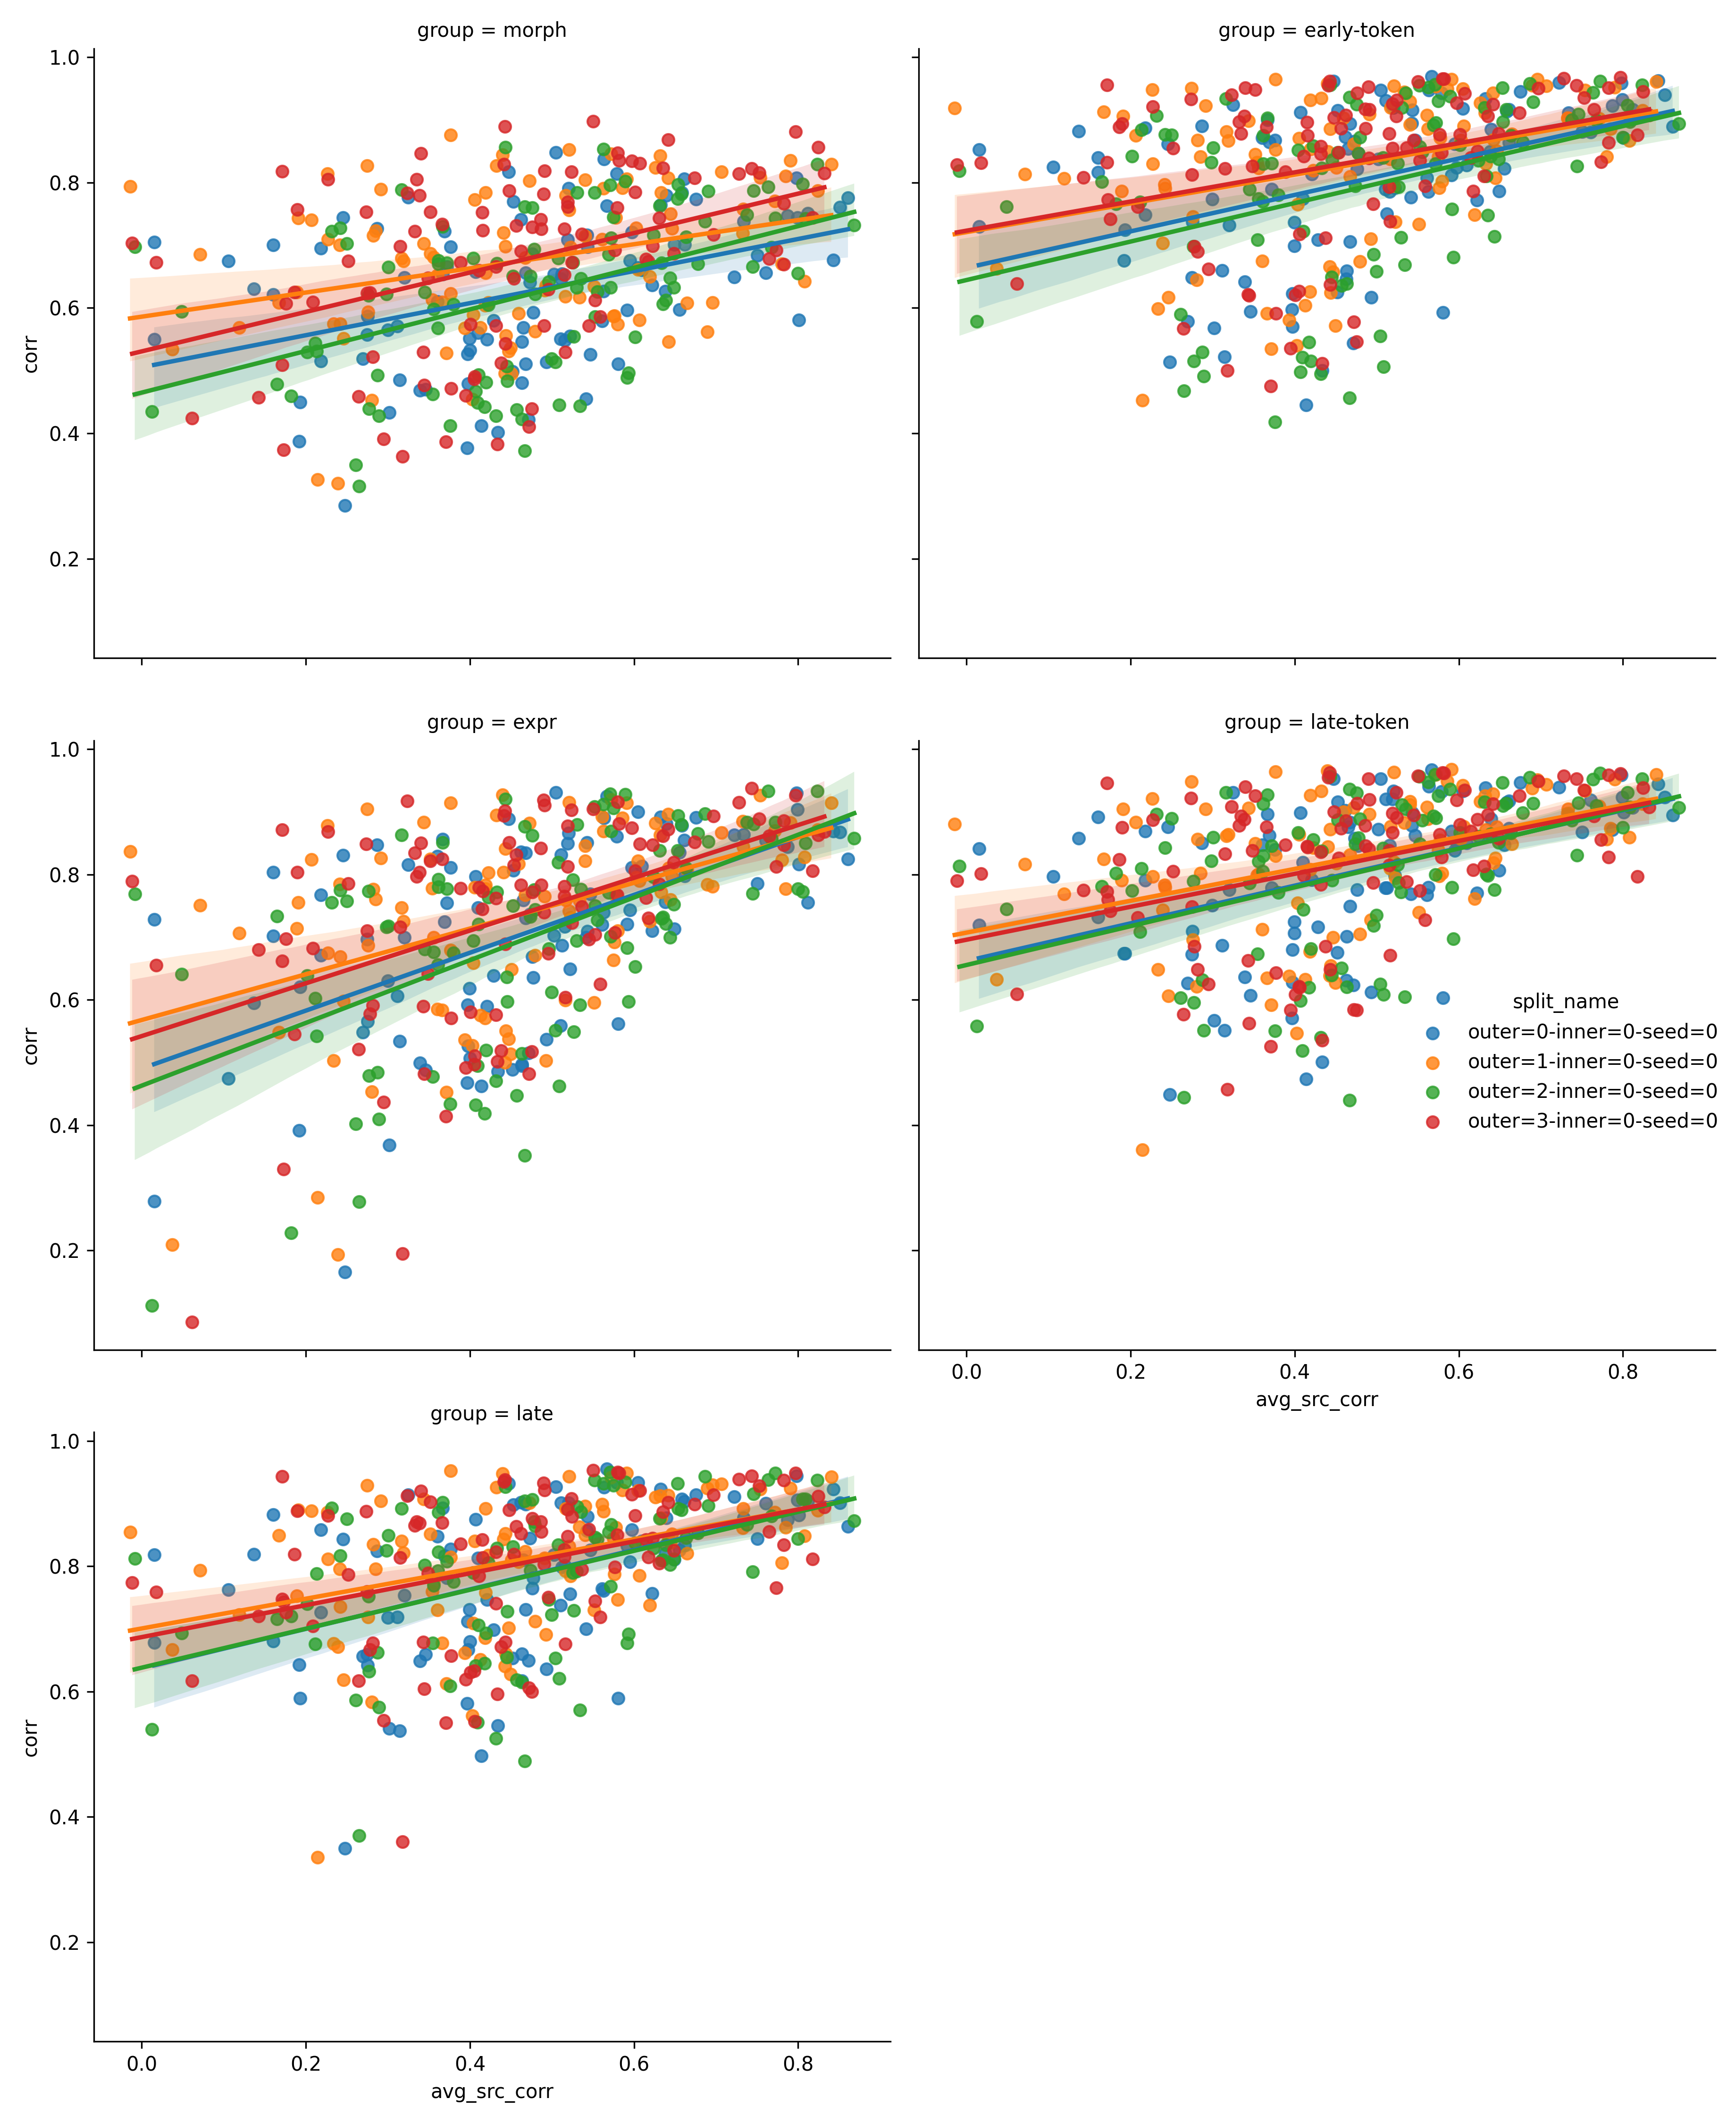
\includegraphics[width=0.95\linewidth]{figures/avg_src_corr_vs_performance-scatterplot.png}
  \caption{\textbf{Predictability vs.\ redundancy with the source panel.} Per-target prediction performance as a function of \texttt{avg\_src\_corr}, the average correlation of a target gene to all genes in the source (core) panel. Higher \texttt{avg\_src\_corr} indicates stronger redundancy with the source panel and is associated with improved predictability. Points are colored by gene program annotations, demonstrating that prediction difficulty varies systematically across functional modules.}
  \label{fig:p-fus:avg-src-corr}
\end{figure}

\begin{figure}[t]
  \centering
  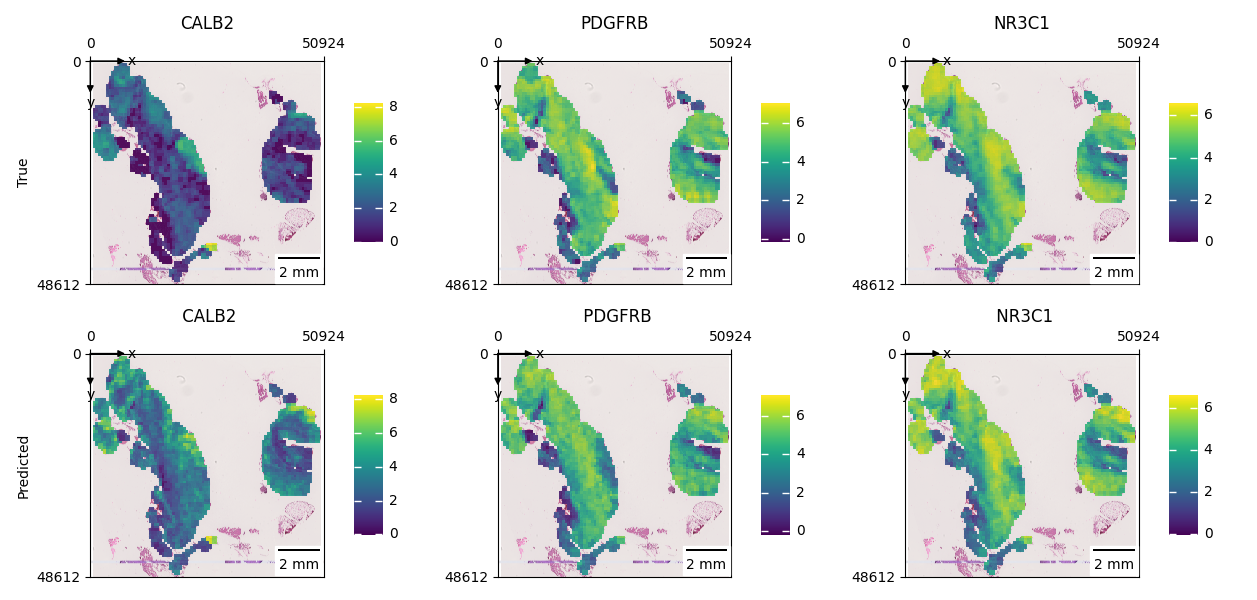
\includegraphics[width=\linewidth]{figures/XE_1H49.04_HNE_1H49-04.png}
  \caption{\textbf{Tile-level predictions on one example sample.} Predicted versus true expression values per tile for the late fusion model. Three representative genes are shown to span the within-sample performance distribution: CALB2 (lowest correlation), PDGFRB (median correlation), and NR3C1 (highest correlation). Each point represents a single tile, with the diagonal indicating perfect prediction. The late fusion model captures expression patterns well across the dynamic range, with performance varying by gene as expected from their source panel correlations.}
  \label{fig:p-fus:true-vs-predicted}
\end{figure}


\begin{figure}[t]
  \centering
  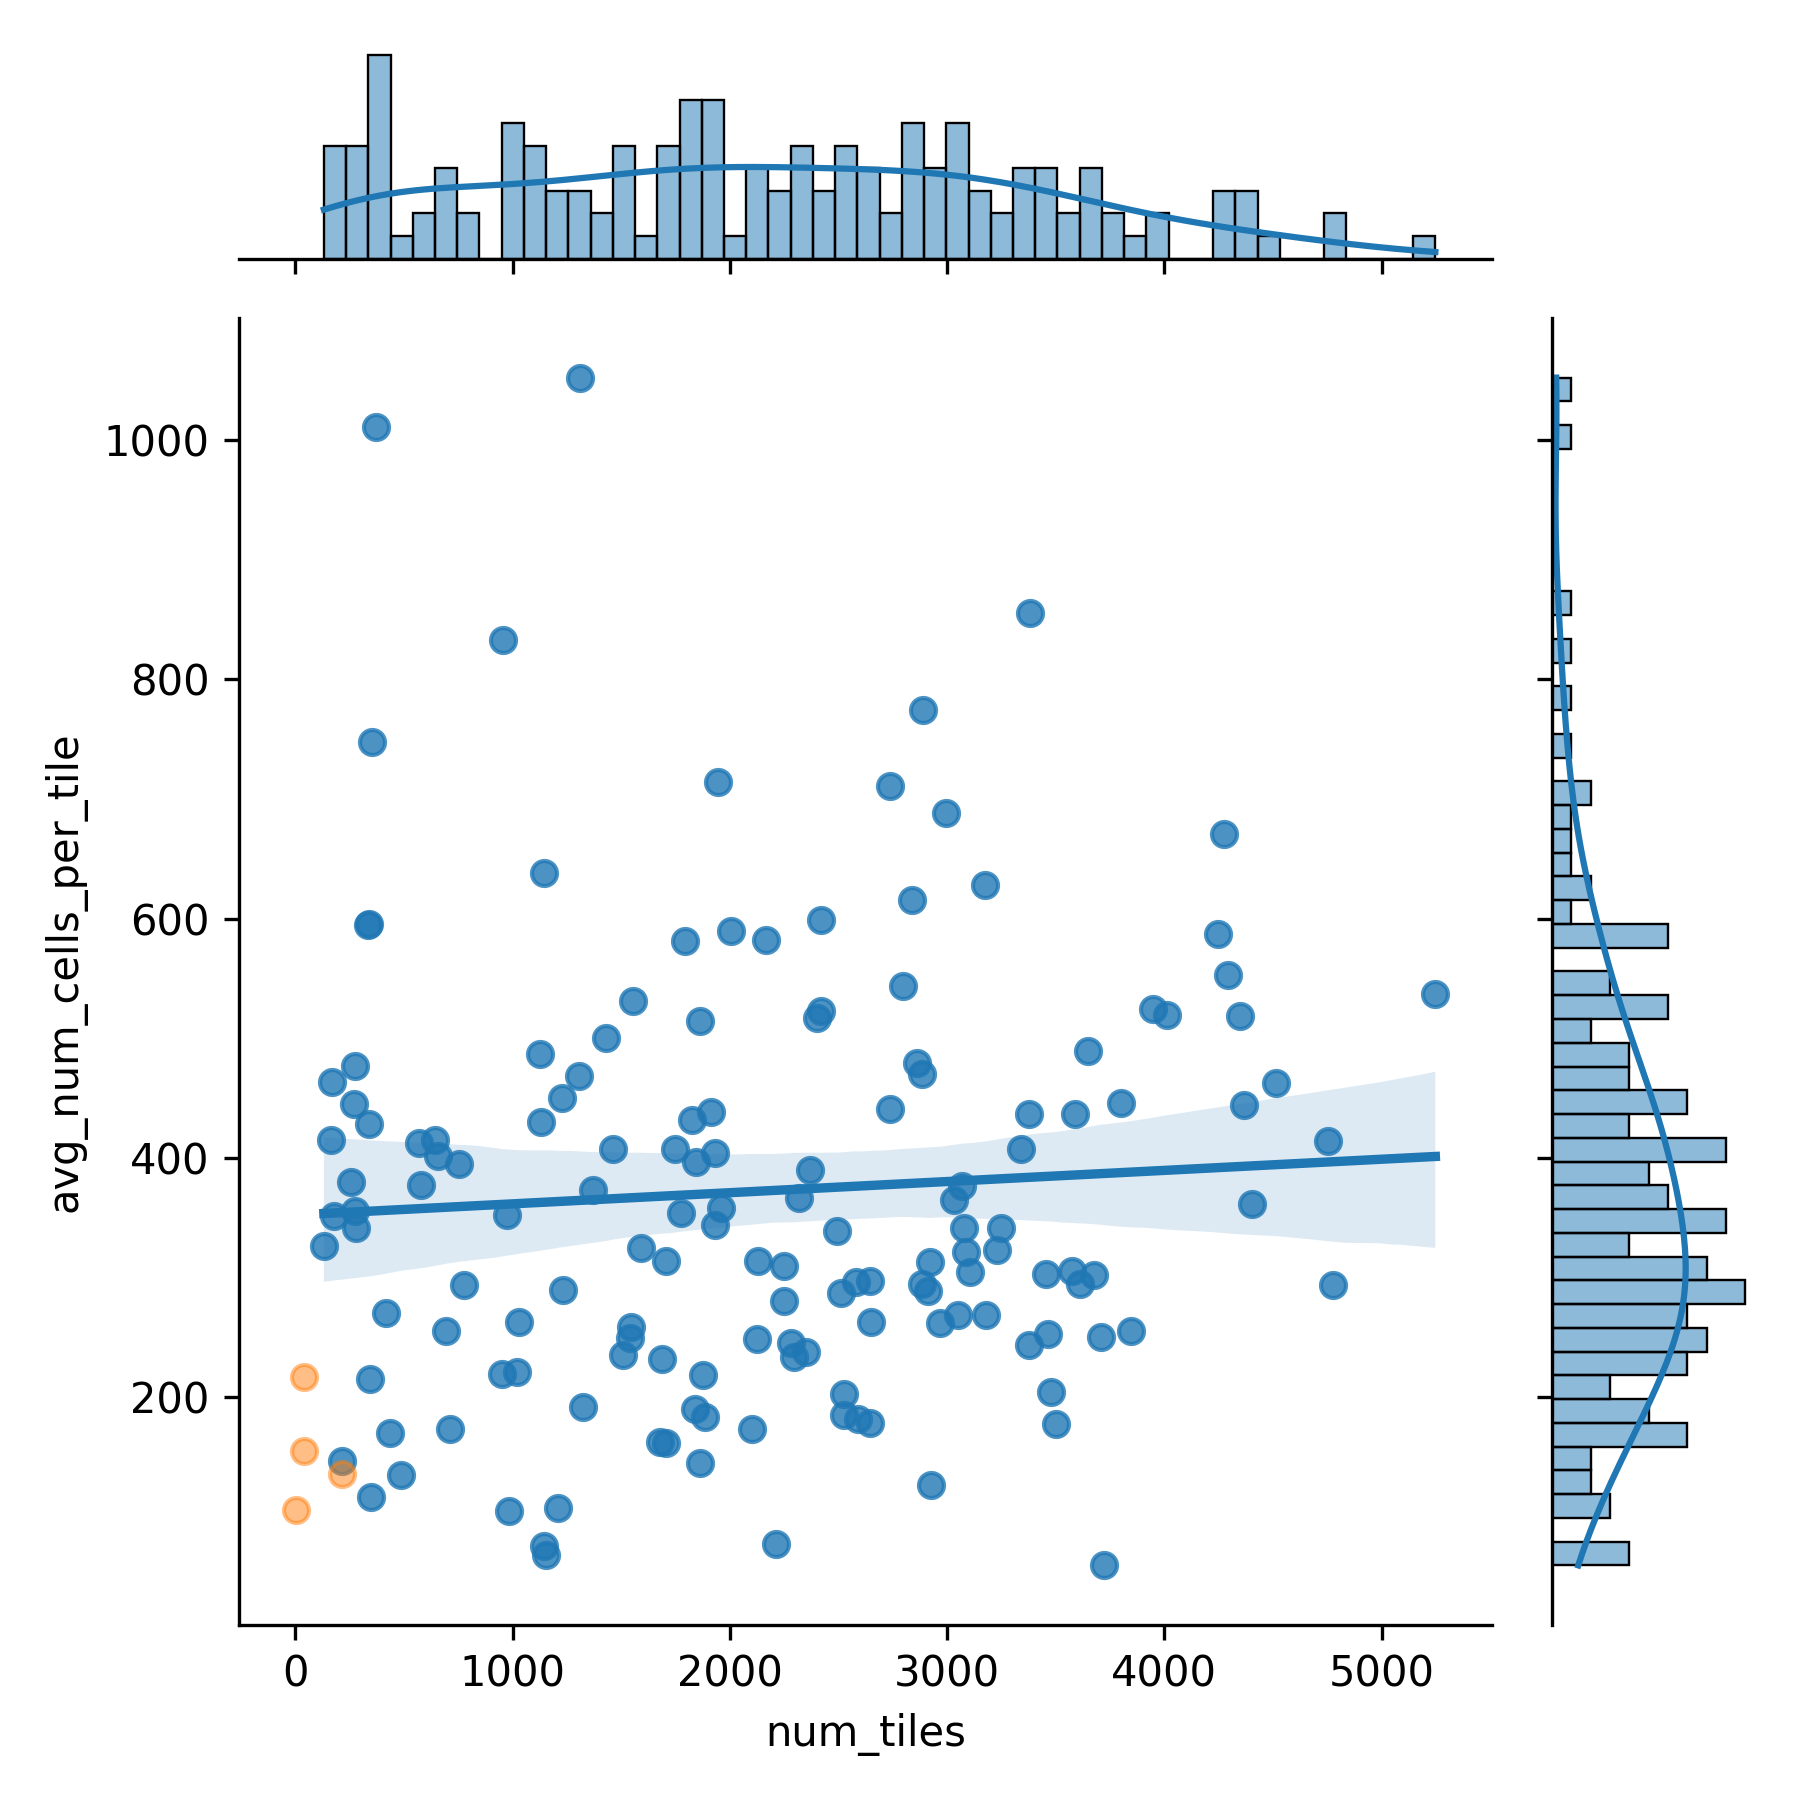
\includegraphics[width=0.8\linewidth]{figures/appendix/num_tiles_vs_avg_num_cells_per_tile.png}
  \caption{\textbf{Cell density is independent of whole-slide image size.} Relationship between the number of tiles per sample (a proxy for WSI size) and the average number of cells per tile (cell density). The lack of correlation indicates that cell density is a tissue-intrinsic property rather than an artifact of tissue section size or processing, supporting the validity of cross-sample comparisons. Each point represents one patient sample.}
  \label{fig:p-fus:tiles-vs-density}
\end{figure}

\begin{figure}[t]
  \centering
  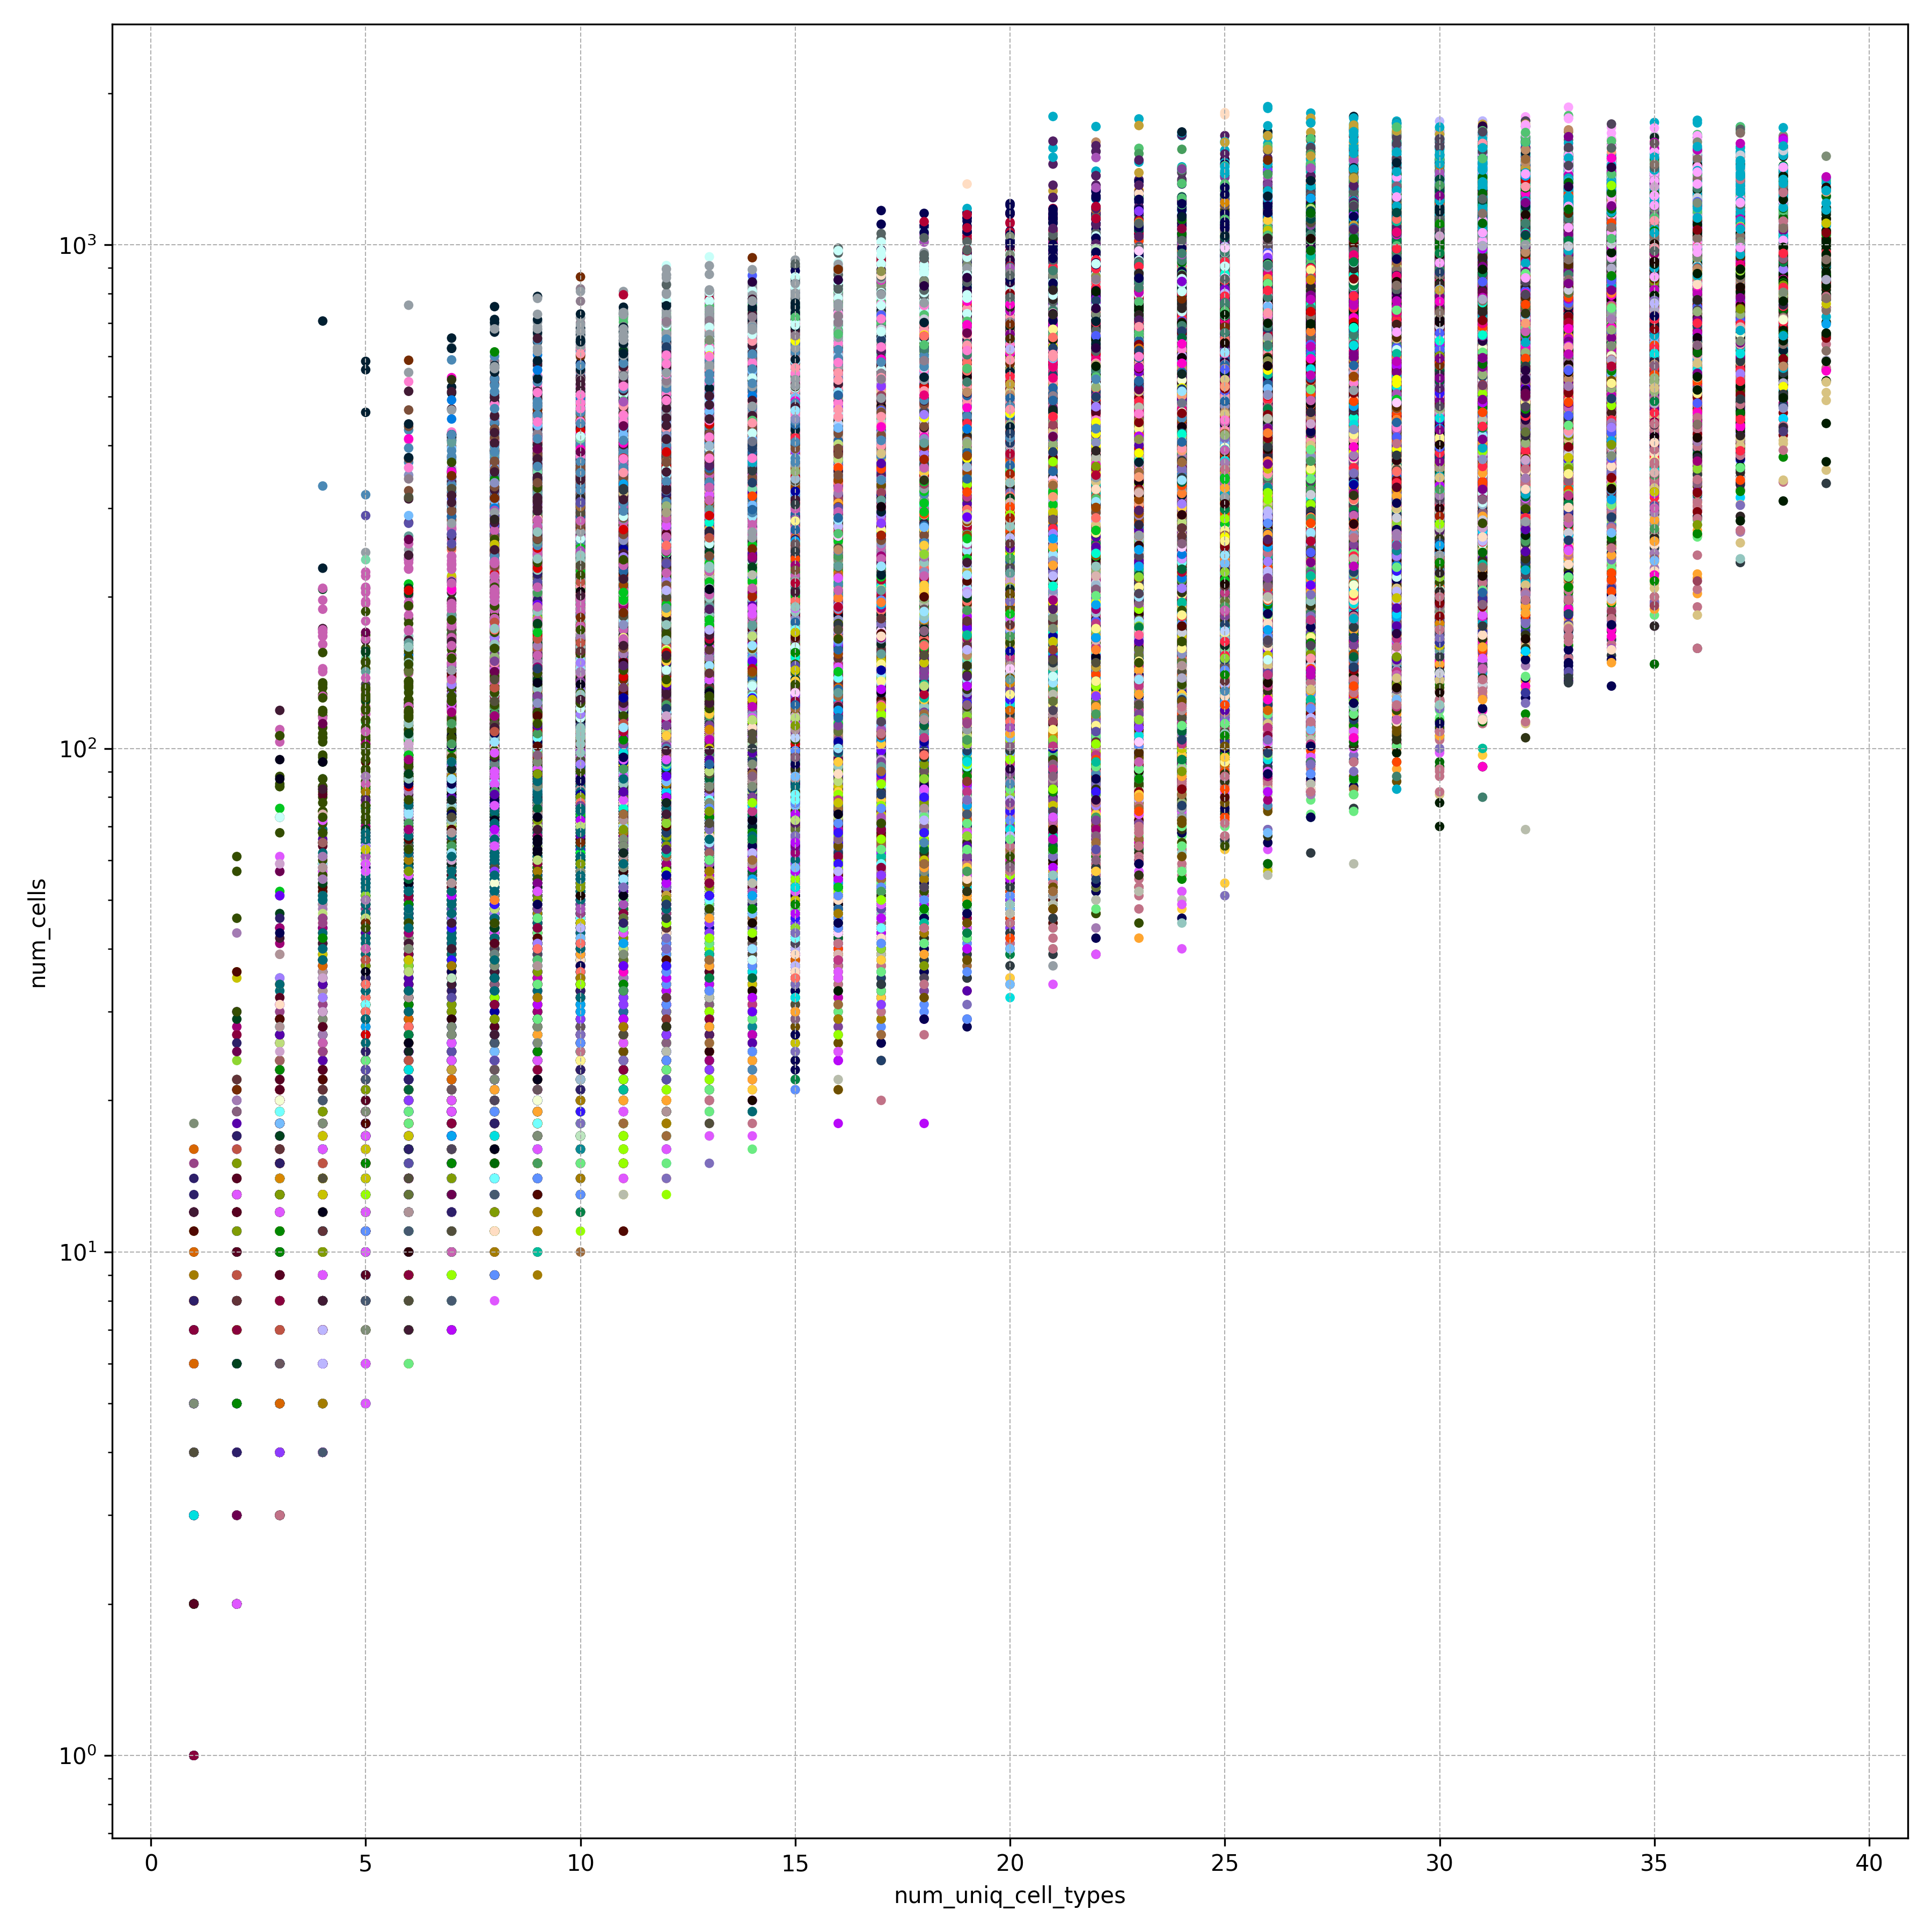
\includegraphics[width=0.8\linewidth]{figures/appendix/num_uniq_cell_types_vs_num_cells_in_tiles-hue=sample_id.png}
  \caption{\textbf{Cell type diversity increases with cell count per tile.} Relationship between the number of cells in a tile and the number of unique cell types detected, colored by sample ID. Tiles with more cells tend to capture greater cell type diversity, reflecting the increased likelihood of sampling rare cell types in regions with higher cellularity. The consistent trend across samples (different colors) demonstrates that this relationship is robust across the cohort.}
  \label{fig:p-fus:cell-types-count}
\end{figure}

%\begin{figure}[t]
%  \centering
%  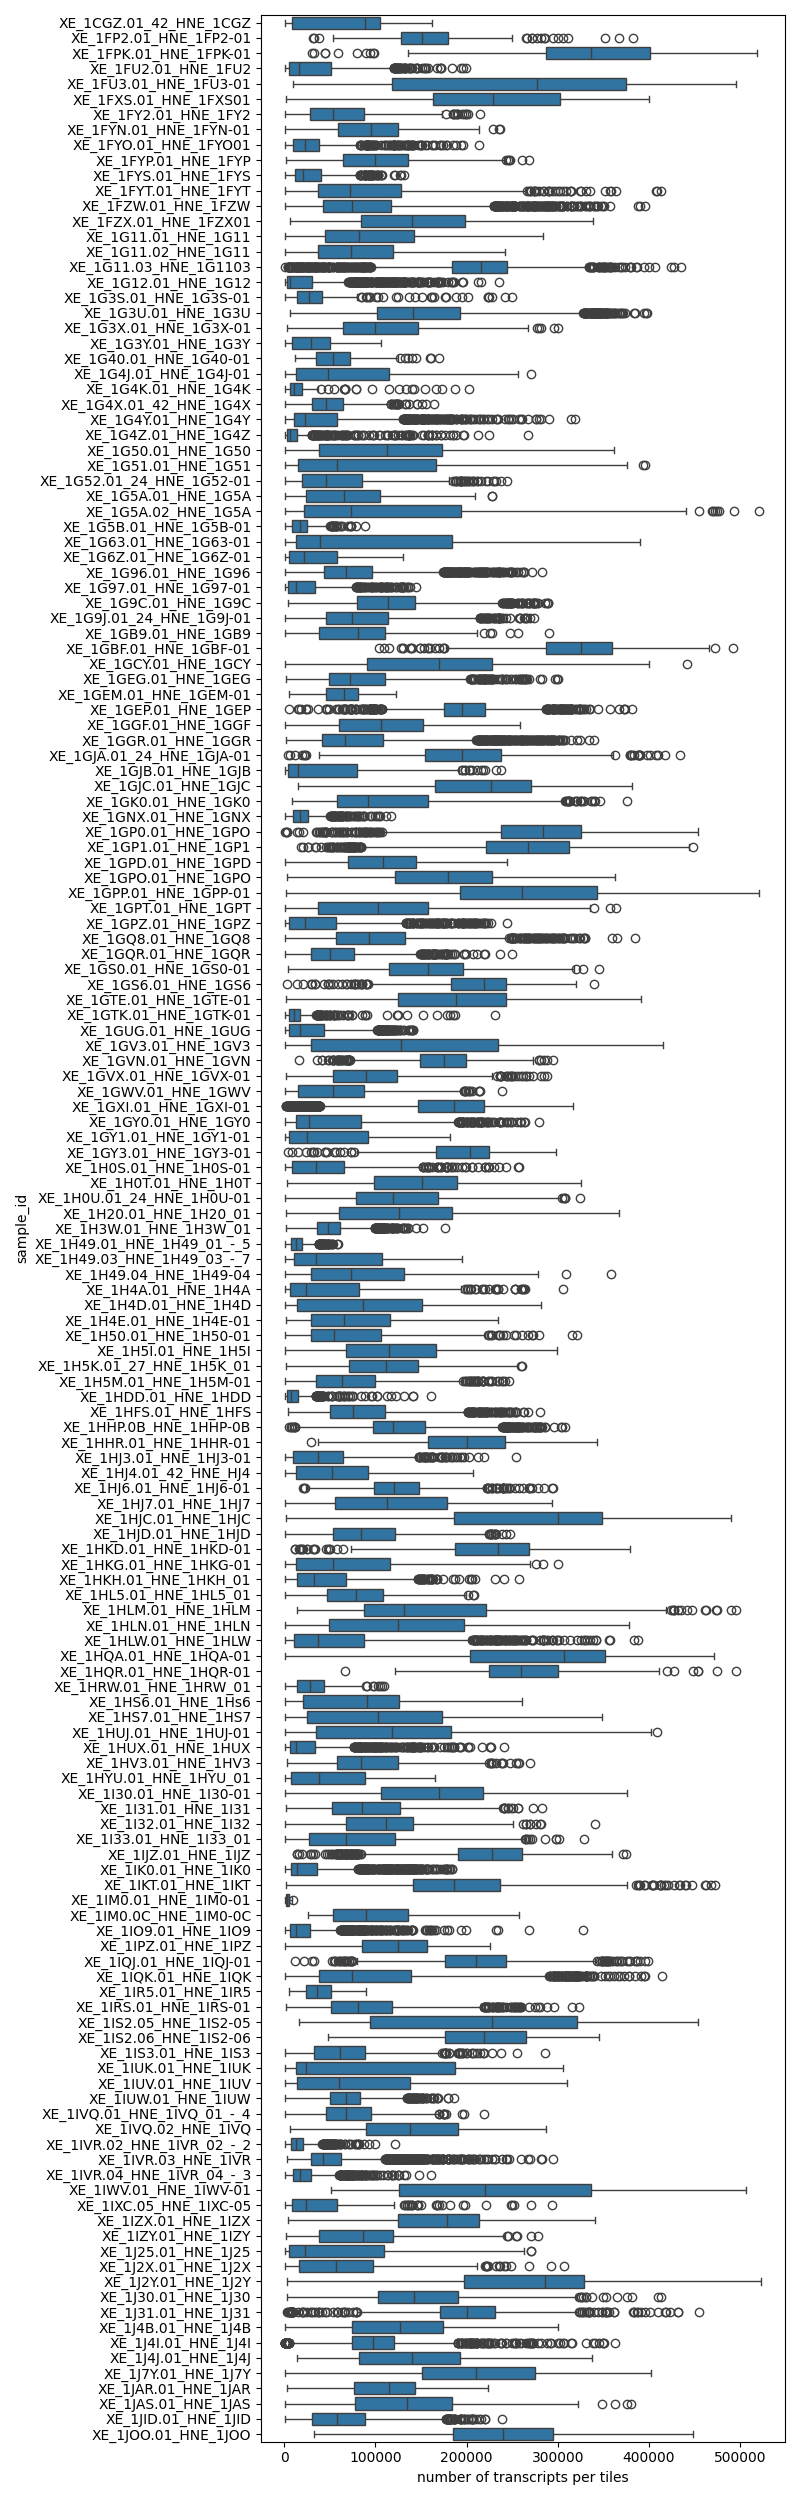
\includegraphics[height=0.8\textheight]{figures/num_transcripts_in_tiles_boxplot.png}
%  \caption{\textbf{Number of transcripts per tile for each sample.}
%  Distribution of transcript counts per tile, shown separately for each patient sample.
%  The substantial inter-sample variability in transcript density motivates the tile-level quality filter
%  requiring at least 1{,}000 transcripts, ensuring sufficient transcriptomic signal for downstream modeling.}
%  \label{fig:p-fus:num-transcripts-in-tiles}
%\end{figure}

\begin{figure}
    \centering
        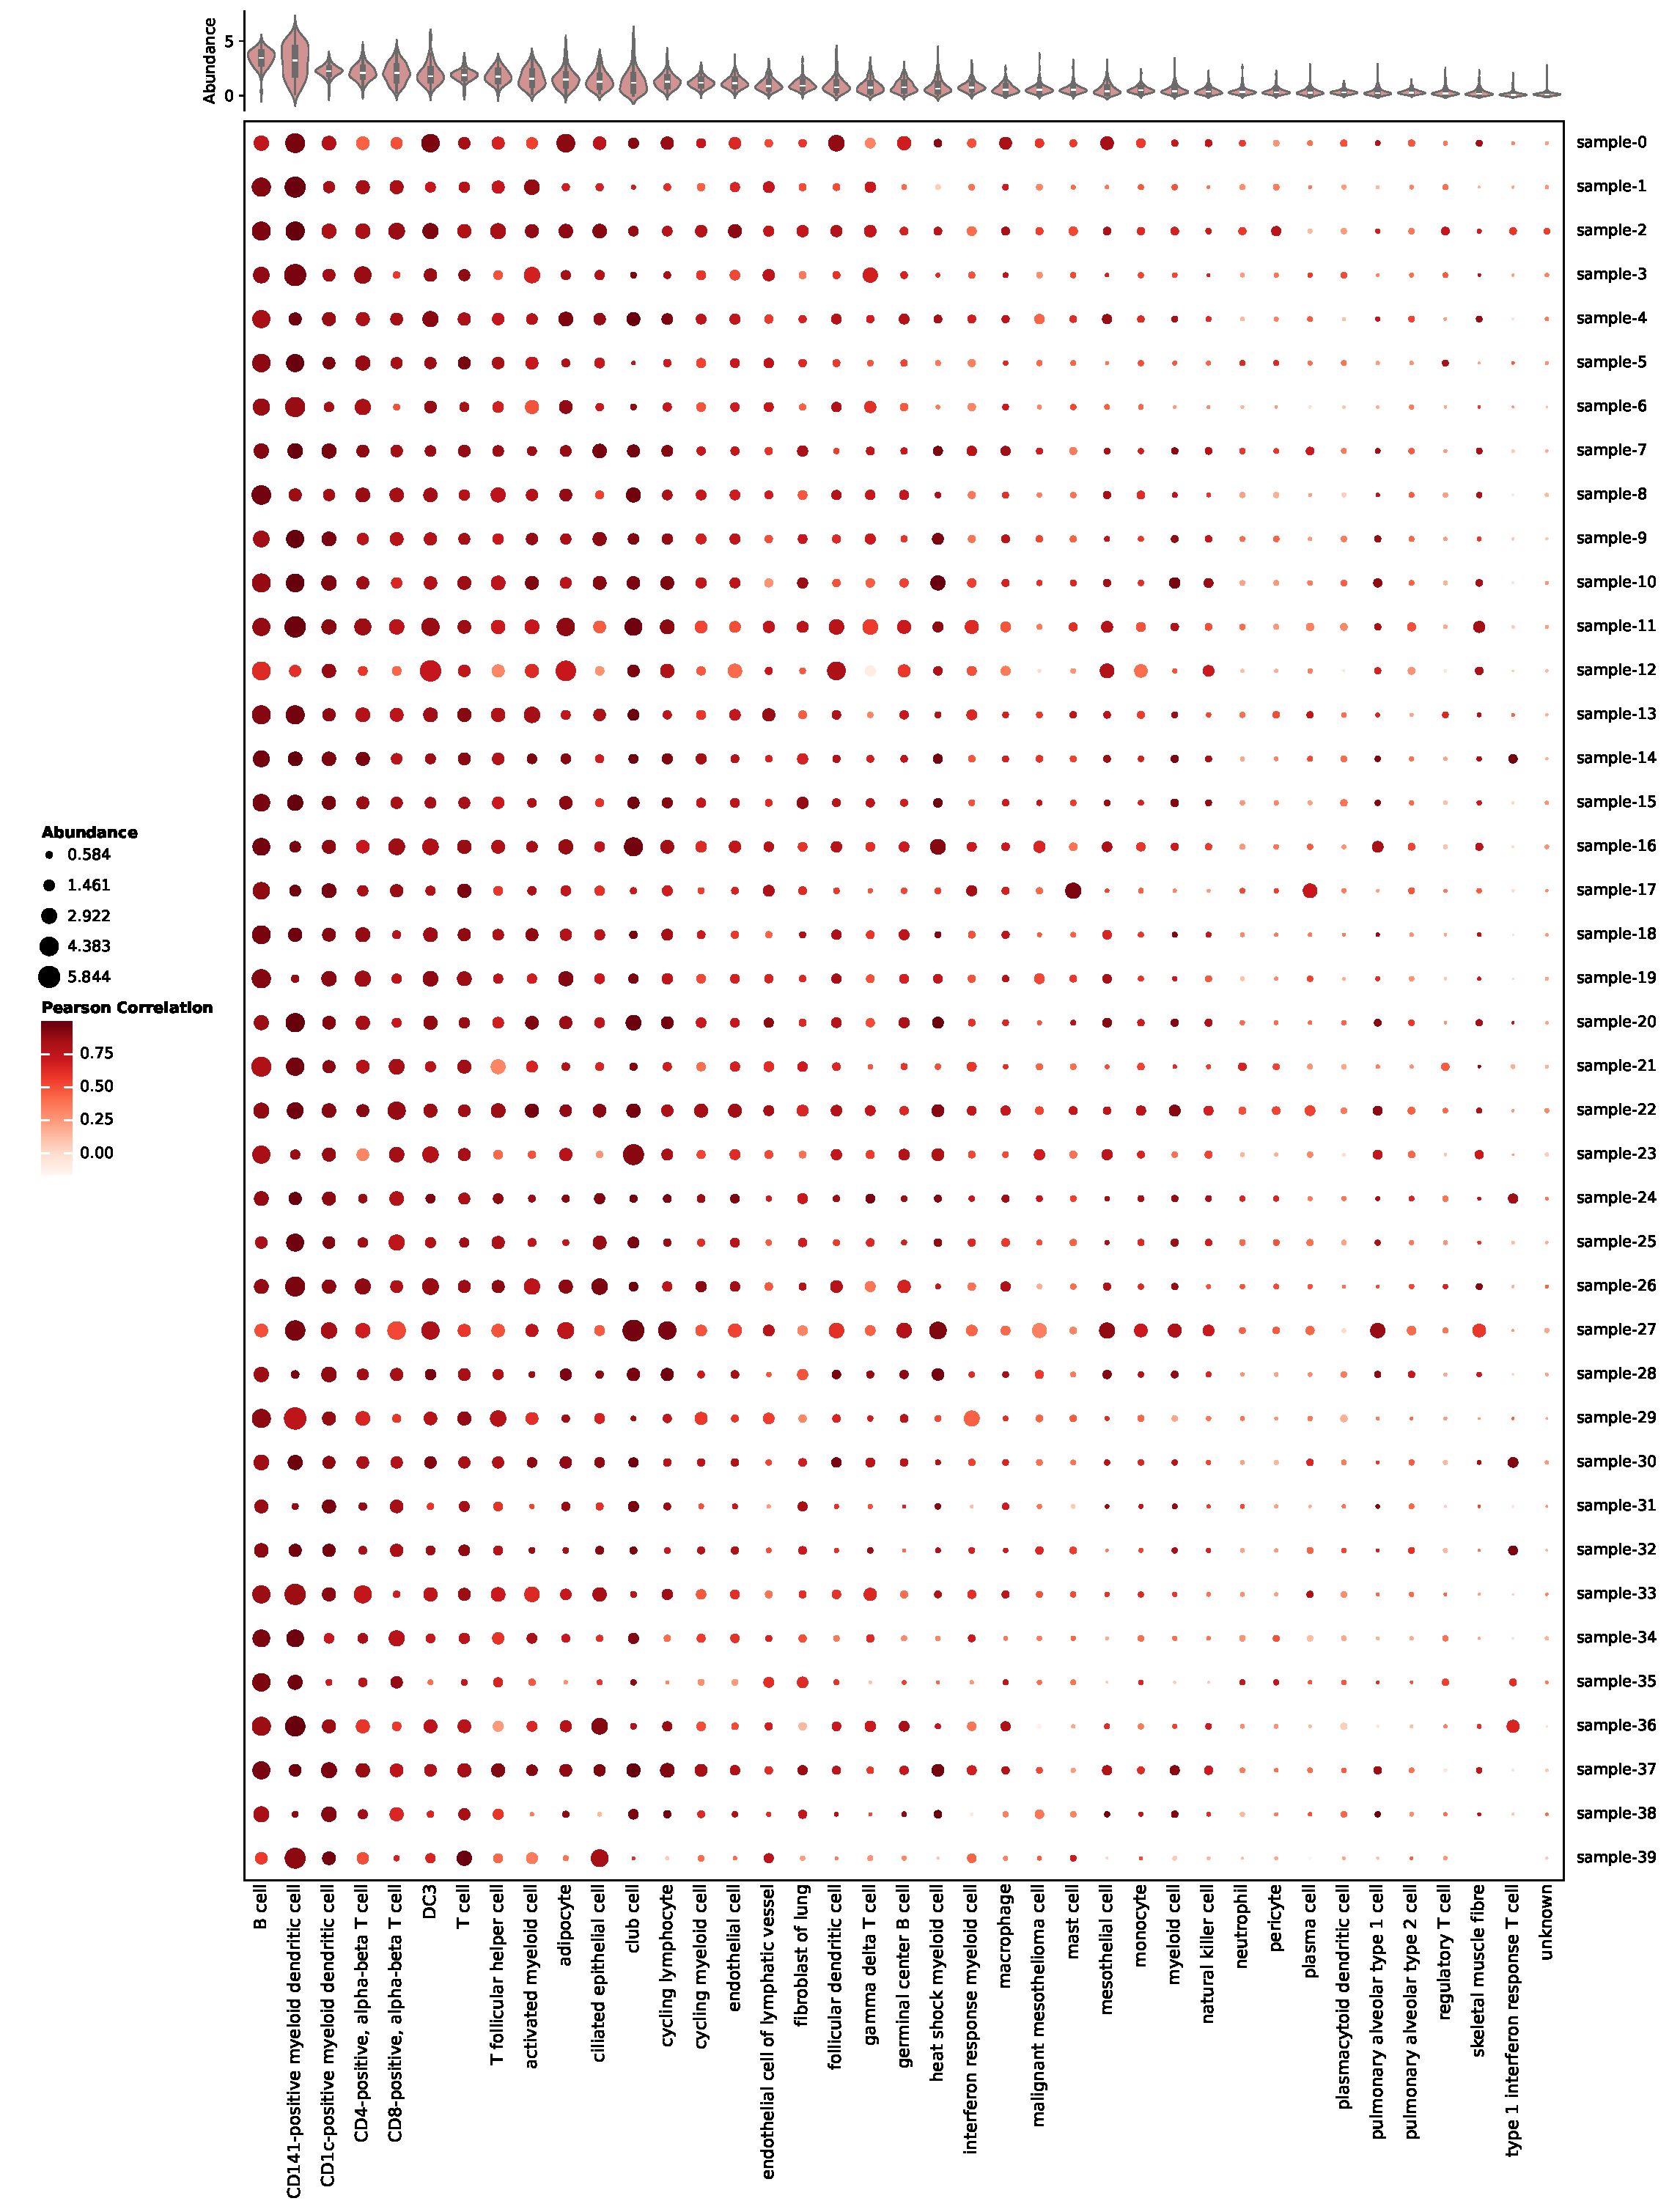
\includegraphics[height=0.8\textheight]{figures/fusion-early-add-mfreeze-0-fusion-sample-level-performance-pearson.pdf}
    \caption{\textbf{Sample-level Pearson correlation for the early-add model.}
    Pearson correlation heatmap for the early-add model on the first data split.
    Rows represent samples ordered by the number of tiles; columns represent cell types ordered by decreasing overall abundance.
    Performance is high and consistent across the majority of abundant cell types (left side), with a gradual decline toward rarer populations (right side), indicating that cell type abundance is the primary driver of per-cell-type predictability.
    No systematic dependence on sample size (number of tiles) is observed.}
    \label{fig:p-fus:sample-level-pearson-2}
\end{figure}
